\documentclass[a4paper,12pt]{report}

\usepackage{alltt, fancyvrb, url}
\usepackage{graphicx}
\usepackage[utf8]{inputenc}
\usepackage{float}
\usepackage{hyperref}
\usepackage{amsmath,amsthm}
\usepackage{amsfonts}
\usepackage[charter]{mathdesign}
\usepackage{booktabs}
\usepackage{makecell}
\usepackage{array}
\usepackage{lscape}
\usepackage{rotating}
\usepackage{tabto}
\usepackage{enumitem}
\usepackage{threeparttable}
\usepackage[italian]{babel}
\usepackage[italian]{cleveref}

\aboverulesep=0ex
\belowrulesep=0ex
\renewcommand{\cellalign}{l}

%------------------------------------------------------

\begin{document}

\begin{titlepage}
    \begin{center}
        \title{}
        {\Huge\bfseries Progetto di Basi di Dati\\per la gestione di un'attività\\in ambito trashware}\\
        \vspace{1cm}
        {\Large Elena Boschetti}\\
        \vspace{1cm}
        {\Large \today}\\
        \vspace{1cm}
        {\Large A.A. 2023/2024}\\
        \vspace{1cm}
        \begin{list}{}{
            \setlength{\leftmargin}{1.5in}
            \setlength{\labelwidth}{0pt}
            \setlength{\labelsep}{1in}
            \setlength{\itemsep}{5pt}}
            \raggedright
            \item[\hbox to 0pt{Matricola:}] {0001020356}
            \item[\hbox to 0pt{E-mail:}] {elena.boschetti@studio.unibo.it}
        \end{list}
    \end{center}
\end{titlepage}

%------------------------------------------------------

\begin{abstract}

\noindent \textbf{Trashware Cesena}\footnote{\url{https://www.trashwarecesena.it/}} è un progetto dell'associazione studentesca S.P.R.I.Te.\footnote{\url{https://sprite.csr.unibo.it/}} dedito al \textit{trashware}\footnote{\url{https://it.wikipedia.org/wiki/Trashware}}: si occupa, cioè, di recuperare dispositivi elettronici (nello specifico, personal computer, periferiche e componenti hardware) altrimenti destinati allo smaltimento e di renderli nuovamente operativi, per poi donarli gratuitamente a chi ne ha necessità (privati, enti o aziende).

\noindent Il progetto Trashware riceve i dispositivi attraverso delle donazioni e, a sua volta, effettua delle donazioni a coloro che ne fanno richiesta. \\

\noindent Il sistema creato dovrà supportare le attività del progetto Trashware: in particolare, dovrà poter essere utilizzato per la gestione delle donazioni, delle richieste rivolte al progetto Trashware e dell’inventario dei dispositivi.

\end{abstract}

%------------------------------------------------------

\tableofcontents

%------------------------------------------------------

\chapter{Analisi dei requisiti}

\section{Intervista}

Innanzitutto, si vuole che il sistema consenta di registrare le donazioni ricevute ed effettuate dal progetto Trashware.
\\\\
I dispositivi che sono oggetto delle donazioni effettuate e ricevute dal progetto Trashware sono personal computer (desktop e portatili), periferiche e singoli componenti. 
\\\\
Il donatore o il donatario possono essere enti (come scuole e associazioni), aziende o privati. \\
Essi devono sempre fornire le generalità e i contatti di una persona che ha il ruolo di referente nell'ambito dell'operazione; nello specifico, le generalità da fornire sono codice fiscale, nome, cognome, data e luogo di nascita, luogo di residenza (città, CAP, provincia, via, numero civico), mentre come contatti deve essere almeno fornito un numero di telefono; opzionalmente, possono essere forniti anche un altro numero di telefono, un numero di fax e un indirizzo e-mail. \\
Se il donatore o donatario è un privato, allora si considera egli stesso come referente. Se invece il donatore o donatario è un ente o un'azienda, allora deve nominare una persona come referente, che ha quindi il ruolo di intermediario tra progetto Trashware e l'ente o l'azienda. In tal caso, devono essere anche forniti il nome, la partita IVA, il codice fiscale e la sede legale (città, CAP, provincia, via, numero civico) dell'ente o dell'azienda e il ruolo del referente all'interno di essa.
\\\\
Sia per effettuare una donazione, sia per richiederla, il donatore o donatario deve fornire:
\begin{itemize}
	\item i dati sopra indicati del referente e dell'ente o azienda di cui esso è eventualmente intermediario;
	\item un elenco che descriva brevemente i dispositivi che sono oggetto della donazione o richiesta;
	\item eventuali note contenenti informazioni legate alla donazione.
\end{itemize}
Nel caso di una richiesta di donazione, il donatario deve anche specificare l’uso che intende fare dell'attrezzatura ricevuta. \\

\noindent I dettagli riguardanti il dispositivo che vengono riportati a livello di inventario sono elencati alla fine di questa sezione. Tali informazioni vengono raccolte dall'operatore del progetto che, a seguito della donazione, si occupa dell'analisi dei dispositivi e della loro registrazione. 
\\\\
A seguito di una richiesta di donazione, deve poter essere registrato nel sistema un ordine che memorizzi i dettagli della richiesta, comprensivi della data della richiesta e della data entro la quale la consegna deve essere effettuata. Ad ogni ordine viene assegnato un livello di priorità e si tiene inoltre traccia dello stato dell’ordine (in lavorazione, pronto, consegnato). Il giorno in cui i dispositivi sono pronti per la consegna, se ne registra la data, e si registra anche la data della consegna una volta che è stata effettuata.
\\\\
Il donatario può poi rivolgersi nuovamente al progetto Trashware in caso di guasti o altri problemi legati ai dispositivi ricevuti. In tal caso, il donatario effettua una richiesta di manutenzione, specificando quali sono i dispositivi interessati e fornendo una descrizione del problema verificatosi ed eventuali altre note utili. Anche in questo caso, il donatario deve fornire generalità e contatti di un referente per l'interazione con l'associazione. Come per le richieste di donazione, le informazioni legate alla richiesta di manutenzione vengono registrate nel sistema insieme alla sua data di effettuazione e alla sua deadline; si mantengono aggiornati il suo stato di lavorazione e il suo livello di priorità e, una volta restituiti i dispositivi, si registra la data della consegna.

\subsection{Informazioni sui dispositivi riportate in inventario} \label{Inventario}

A livello di inventario, devono essere registrate le seguenti informazioni sui dispositivi. \\
Per prima cosa, ad ogni dispositivo si associa un codice identificativo. \\
A seconda della tipologia del dispositivo, devono poi essere visualizzabili le seguenti informazioni.
\begin{itemize}
	\item Per \textbf{singoli componenti}:
		\begin{itemize}
			\item \textbf{per ogni tipologia di componente:} tipo, marca e modello;
			\item \textbf{CPU:} architettura;
			\item \textbf{RAM:} dimensione (in GB);
			\item \textbf{Memoria di massa:} tipologia (HDD o SSD) e dimensione (in GB);
			\item \textbf{Chassis:} colore.
		\end{itemize}
	\item Per le \textbf{periferiche}:
		\begin{itemize}
			\item \textbf{per tutti i tipi di periferiche:} tipo, marca, modello e tipologia di connettività (wired o wireless).
			\item Solo per i \textbf{monitor:}
				\begin{itemize}
					\item tipologia (es. CRT, LCD)
					\item dimensioni (in pollici);
					\item aspect ratio (es. 16:9);
					\item disponibilità di connettività VGA e/o DVI;
					\item disponibilità di audio integrato.
				\end{itemize}
		\end{itemize}
	\item Per i \textbf{PC}, sia desktop sia portatili:
		\begin{itemize}
			\item informazioni sopra indicate legate a CPU;
            \item quantità di RAM;
            \item informazioni sopra indicate legate alla memoria di massa (1 o 2 unità);
			\item sistema operativo installato, versione e data del suo ultimo aggiornamento;
			\item disponibilità di connettività Ethernet, WiFi e Bluetooth.
		\end{itemize}
	\item Solo per i \textbf{PC desktop}:
		\begin{itemize}
			\item informazioni sopra indicate legate allo chassis;
			\item identificativi di monitor, tastiera, mouse e casse audio se forniti insieme al PC desktop.
		\end{itemize}
	\item Solo per \textbf{PC portatili}:
		\begin{itemize}
			\item marca e modello del PC;
			\item dimensioni dello schermo (in pollici);
			\item colore del telaio.
		\end{itemize}
\end{itemize}
\noindent Si possono infine inserire eventuali note riguardo al dispositivo.


\section{Estrazione dei requisiti}

A seguito dell'intervista, si procede ad una riformulazione delle informazioni ottenute che renda più semplice la modellazione concettuale del dominio descritto. In particolare, si effettua prima l'estrazione dei concetti principali del dominio, anche con l'obiettivo di eliminare le ambiguità presenti. Questa operazione rende più facile la successiva formalizzazione dei requisiti, i quali devono essere esposti in maniera quanto più chiara e ordinata.

\subsection{Estrazione dei concetti principali}

\newcolumntype{A}{>{\raggedright\arraybackslash}p{0.6\linewidth}}
\newcolumntype{B}{>{\raggedright\arraybackslash}p{0.2\linewidth}}
\begin{table}[H]
	\begin{center}
	    	\begin{tabular}{B|A|B}
    	      	\toprule
    	      		\textbf{Termine} & \textbf{Descrizione} & \textbf{Eventuali sinonimi}\\
    	      	\midrule
    					Referente
    					& Persona che agisce da intermediario nell'ambito della richiesta o donazione effettuata al progetto Trashware. Se la richiesta o la donazione proviene da un ente o un'azienda, il referente corrisponde all'intermediario da esso nominato per la collaborazione; se invece la richiesta o donazione è effettuata da un privato, il referente è il privato stesso.
    					& Donatore / donatario (quando è un privato)\\
    					% ----------------------
    					\hline
    					Società
    					& Qualora la richiesta o donazione provenga da un ente o da un'azienda, si indica con il termine "società" tale ente o azienda.
    					& Ente, azienda, donatore / donatario (quando è un ente o un azienda)\\
    					% ----------------------
    					\hline
    					Richiesta
    					& Richiesta di una donazione o di manutenzione di dispositivi per la quale un cliente si rivolge al progetto Trashware.
    					& Ordine (richiesta di donazione) \\
    					% ----------------------
    					\hline
    					Donazione
    					& Donazione di dispositivi che sono devoluti al progetto Trashware.
    					& \\
    					% ----------------------
                        \hline
                        Operazione
                        & Donazione o richiesta effettuata al progetto Trashware.
                        & Donazione, Richiesta \\
                        % ----------------------
    					\hline
    					Dispositivo
    					& PC, periferica o componente che è oggetto di una donazione o di una richiesta effettuata al progetto Trashware.
    					& Attrezzatura \\
    	      	\bottomrule
	    	\end{tabular}
	\end{center}
	\caption{Glossario dei termini, che riporta i concetti principali del dominio.}
    \label{tab:glossary}
\end{table}

\subsection{Riformulazione dei requisiti}

Si vuole realizzare un sistema di basi di dati che supporti l'attività del progetto Trashware, in particolare per la gestione di ogni richiesta e donazione effettuata al progetto Trashware e per la gestione dell'inventario dei dispositivi.
\\\\
Il donatore o il donatario possono essere enti (come scuole e associazioni), aziende o privati. \\
Essi devono sempre fornire le generalità e i contatti di una persona che ha il ruolo di referente nell’ambito dell’operazione. Nello specifico, le generalità del referente da registrare sono codice fiscale, nome, cognome, data e luogo di nascita, luogo di residenza (città, CAP, provincia, via, numero civico), mentre come contatti viene registrato almeno un numero di telefono e, opzionalmente, un altro numero di telefono, un numero di fax e un indirizzo e-mail. \\
Se il donatore o donatario è un privato, allora si considera egli stesso come referente. Se invece il donatore o donatario è una società (cioè un ente o un'azienda), allora esso deve nominare una persona come referente, che ha quindi il ruolo di intermediario tra progetto Trashware e la società di cui è rappresentante. In tal caso, si registrano anche il nome, la partita IVA, il codice fiscale e la sede legale (città, CAP, provincia, via, numero civico) della società e il ruolo che il referente ricopre all'interno di essa.
\\\\
Il donatore o donatario può rivolgersi al progetto Trashware per tre tipi di operazione: per devolvere dei dispositivi (donazione), per richiedere una donazione di dispositivi (richiesta di donazione) o per richiedere un intervento di manutenzione su dispositivi ricevuti in donazione dal progetto (richiesta di manutenzione).
\\
Nell'ambito di tutte le tre tipologie di operazione, si registrano:
\begin{itemize}
	\item i dati sopra indicati del referente e della società di cui esso è eventualmente intermediario;
	\item un elenco che descriva brevemente i dispositivi che sono oggetto dell'operazione;
	\item la data in cui viene effettuata l'operazione;
	\item eventuali note riguardanti l'operazione.
\end{itemize}

\noindent Nell'ambito delle richieste (di donazione o di manutenzione):
\begin{itemize}
	\item si registra anche la data entro la quale i dispositivi devono essere pronti;
	\item viene assegnato un livello di priorità alla richiesta;
	\item viene memorizzato e mantenuto aggiornato lo stato della richiesta (in lavorazione, pronto, consegnato);
	\item il giorno in cui i dispositivi sono pronti per la consegna, se ne registra la data;
	\item una volta che i dispositivi sono stati consegnati, si registra la data della consegna.
\end{itemize}
\noindent Inoltre, nel caso di una richiesta di donazione viene anche specificato l’uso che il donatario intende fare dei dispositivi ricevuti, mentre nel caso di una richiesta di manutenzione viene registrata anche una descrizione del problema che si è verificato.
\\\\
Per quanto concerne la gestione dell'inventario, si evidenzia che le informazioni riguardanti un dispositivo ricevuto vengono raccolte dall'operatore del progetto che, a seguito della donazione, si occupa dell'analisi dei dispositivi e della loro registrazione.
\\
Le informazioni da registrare per ogni tipologia di dispositivo sono elencate nella sottosezione \ref{Inventario} proposta in precedenza.

\subsection{Operazioni principali} \label{Operazioni}

Le principali operazioni che si vorranno effettuare sul sistema sono le seguenti.

\begin{itemize}
	\item Registrazione di una nuova donazione devoluta al progetto, registrando anche tutte le informazioni relative al referente e alla società di cui è eventualmente rappresentante
	\item Visualizzazione delle donazioni devolute al progetto e delle relative informazioni in merito al richiedente
    \item Registrazione di una nuova richiesta effettuata al progetto, registrando anche tutte le informazioni relative al referente e alla società di cui è eventualmente rappresentante
	\item Visualizzazione delle richieste, divise in base al loro stato corrente ed elencate in ordine decrescente di priorità
	\item Aggiornamento dello stato di una richiesta e registrazione del suo completamento e della sua consegna
	\item Inserimento di un nuovo dispositivo nell'inventario, specificando tutti i dati caratterizzanti il dispositivo in oggetto
    \item Visualizzazione delle informazioni sui dispositivi registrati in inventario (compresi i dispositivi assegnati ad una richiesta), filtrando per tipologia di dispositivo
	\item Associazione di un dispositivo ad un'operazione (alla donazione con la quale è stato ricevuto, alla richiesta di donazione per la quale viene donato e alle eventuali richieste di manutenzione che lo riguardano)
    \item Associazione di un componente ad un PC o di una periferica ad un PC desktop
\end{itemize}

%------------------------------------------------------

\chapter{Progettazione concettuale}

\section{Schema scheletro e raffinamenti proposti}

A seguito dell'analisi del dominio, si può pervenire al seguente schema scheletro:

\begin{figure}[H]
	\centering
	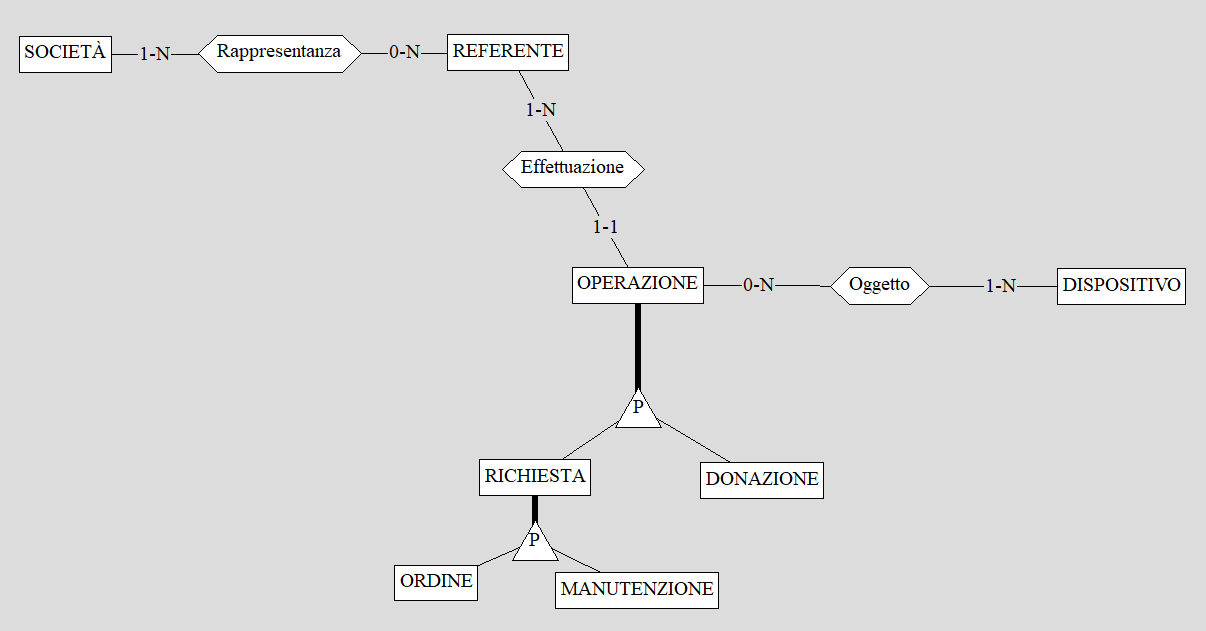
\includegraphics[width=\textwidth]{images/schema-scheletro.png}
	\caption{Schema E-R contenente le entità e associazioni principali del dominio.}
	\label{images:schema-scheletro}
\end{figure}

\noindent Il \textbf{referente} (identificato dal suo codice fiscale) può essere o meno il rappresentante di una \textbf{società} (identificata dalla sua partita IVA o dal suo codice fiscale), ed è possibile anche che lo sia per differenti società nell'ambito di operazioni distinte. \\
Una società deve invece obbligatoriamente nominare un referente. Nell'ambito di operazioni diverse, può avere referenti diversi. \\
Il titolo del referente indica il suo ruolo all'interno della \textbf{società} di cui è eventualmente rappresentante, per cui è più appropriato come attributo dell'associazione \textbf{Rappresentanza} piuttosto che dell'entità \textbf{Referente}.

\begin{figure}[H]
	\centering
	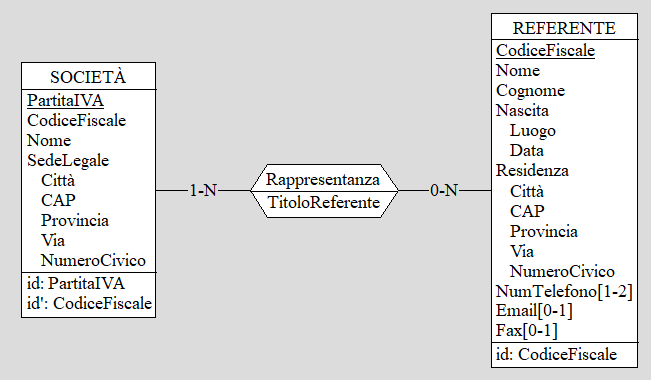
\includegraphics[width=0.7\textwidth]{images/referente.png}
    \caption{Modellazione di referente e società.}
	\label{images:referente}
\end{figure}

\noindent Una \textbf{donazione} devoluta al progetto o una \textbf{richiesta} rivolta al progetto (che può essere un \textbf{ordine} di dispositivi o una richiesta di \textbf{manutenzione}) sono considerate le specializzazioni di una generica \textbf{operazione}. La gerarchia delle operazioni è organizzata in modo da raggruppare le caratteristiche comuni tra le tre tipologie di operazione e tra le due tipologie di richieste. Non essendo presenti proprietà che identifichino univocamente un'operazione, ad essa viene assegnato un codice (\textbf{IDOperazione}). \\
All'operazione viene associato il referente nominato nell'ambito della sua effettuazione. \\
Tra i dati dell'operazione, viene riportato anche un elenco che descrive molto brevemente i dispositivi che sono oggetto dell'operazione. Si evidenzia che le informazioni tecniche sui dispositivi coinvolti vengono acquisite e associate all'operazione solo in un momento successivo alla sua ufficializzazione. Nel caso di un ordine, i dispositivi che verranno donati dovranno essere scelti tra quelli che risultano disponibili consultando l'inventario. \\
Le informazioni tecniche sui dispositivi sono rappresentate dall'entità \textbf{Dispositivo}, la cui modellazione è descritta in seguito. Un'entità \textbf{Dispositivo} può essere associata a più operazioni, poiché un dispositivo viene prima ricevuto tramite una donazione e può poi essere donato a seguito di un ordine ed essere anche eventualmente restituito per motivi di manutenzione.

\begin{figure}[H]
	\centering
	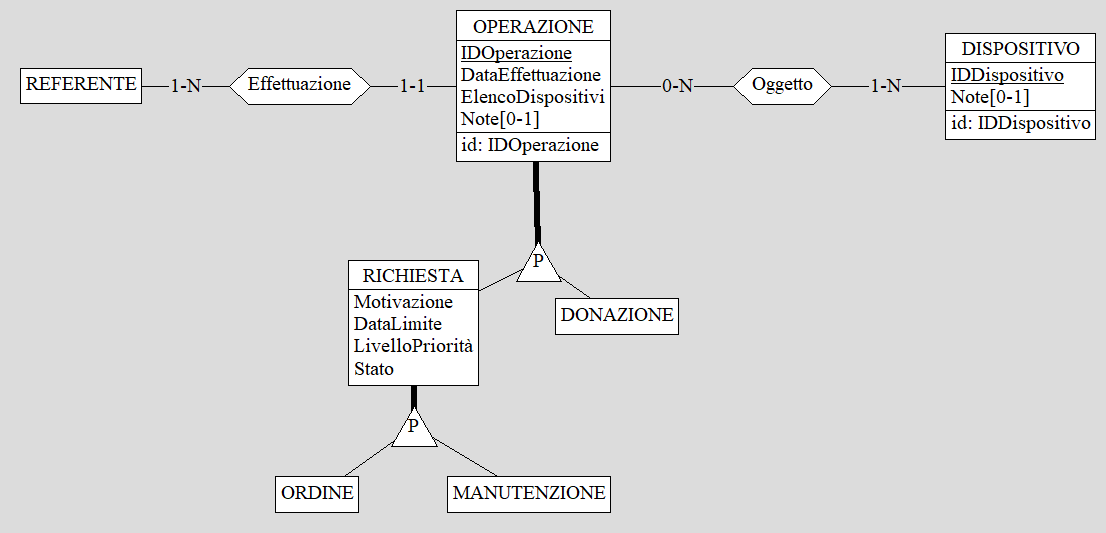
\includegraphics[width=\textwidth]{images/operazione.png}
    \caption{Modellazione delle operazioni.}
	\label{images:operazione}
\end{figure}

\noindent Quando il lavoro legato ad una richiesta viene terminato, si registra la data del suo completamento, così come si registra la data della sua consegna una volta che i dispositivi vengono consegnati. La \textbf{richiesta}, il \textbf{completamento} e la \textbf{consegna} vengono quindi registrati in momenti diversi; inoltre, per ogni richiesta viene registrata una sola data di completamento e, solo in seguito al completamento, viene registrata una sola data di consegna. Per queste motivazioni, ho deciso di modellare il completamento e la consegna come due entità (anche in previsione del fatto che, in futuro, si potrebbero voler registrare altri dati in merito) e di identificarle solo esternamente: il completamento è identificato dalla richiesta a cui fa riferimento, mentre la consegna è identificata dal completamento della richiesta. In questo modo, le due date sono necessariamente uniche, si può registrare la consegna solo nel momento in cui è registrato il completamento e in entrambi i casi è possibile risalire alla richiesta a cui fanno riferimento. Allo stato attuale, si sarebbe potuto anche scegliere di modellare le date come due attributi opzionali della richiesta.

\begin{figure}[H]
	\centering
	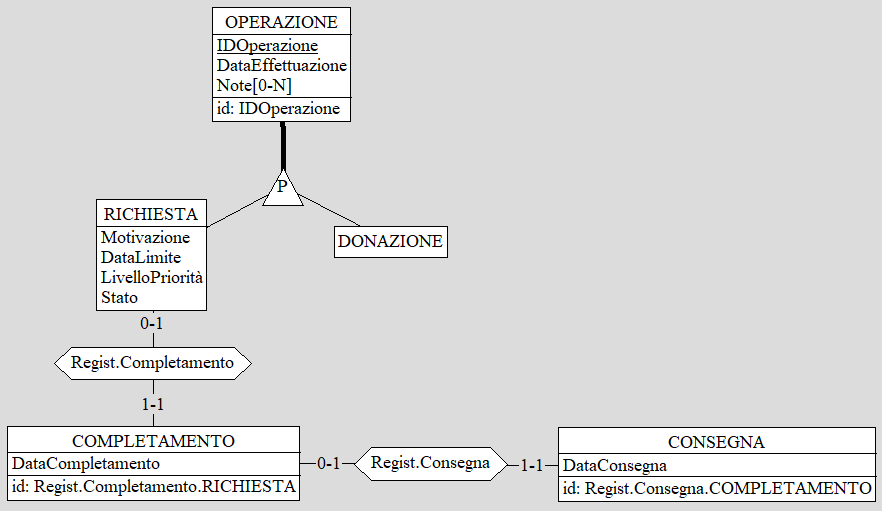
\includegraphics[width=\textwidth]{images/date.png}
    \caption{Modellazione dei completamenti e delle consegne delle richieste.}
	\label{images:date}
\end{figure}

\noindent Per quanto riguarda la modellazione dei dispositivi, data la loro varietà, ho optato per un approccio top-down per individuare le proprietà e i rapporti tra i diversi tipi di dispositivi. Sono prima stati suddivisi nelle tre categorie principali (PC, periferiche, componenti), per poi scendere nella definizione delle diverse sottocategorie e, infine, individuare i rapporti tra dispositivi di categorie diverse (ad esempio, l'associazione tra un PC e i suoi componenti).
\\
Anche in questo caso, si è optato per identificare ogni dispositivo mediante un proprio codice (\textbf{IDDispositivo}): non esiste un insieme di specifiche tecniche che possa identificare univocamente un singolo dispositivo, dato che è possibile che ci siano dispositivi con le stesse specifiche, e assegnare un codice al dispositivo al momento della sua analisi è una scelta accettabilmente comoda.

\begin{figure}[H]
	\centering
	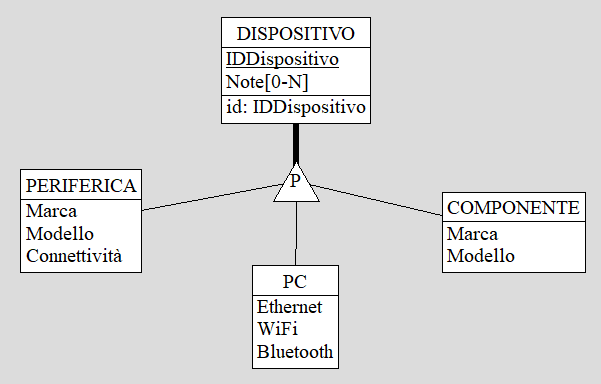
\includegraphics[width=0.5\textwidth]{images/dispositivo.png}
    \caption{Le principali categorie di dispositivi.}
	\label{images:dispositivo}
\end{figure}

\noindent I PC sono distinti in \text{desktop} e \textbf{portatili}. \\
Le due tipologie di PC sono accomunate dalle informazioni in merito ai componenti (l'associazione di tali informazioni è descritta più avanti e mostrata in figura \ref{images:componenti-pc}) e dalle informazioni riguardo alla connettività (Ethernet, Bluetooth, WiFi). \\
I PC desktop sono sempre racchiusi all'interno di uno chassis, il quale è modellato mediante un'entità a sé stante (come mostrato in figura \ref{images:componenti-pc}); in merito al telaio dei PC portatili, invece, è richiesto solo di riportarne il colore. \\
Similmente, ad un PC desktop può essere associato un monitor, modellato come un'entità a sé stante (come mostrato in figura \ref{images:periferiche-pc}); per lo schermo dei PC portatili, invece, è richiesto solo di riportarne la dimensione in pollici. \\
Al contrario dei PC portatili, non è richiesto di registrare marca e modello dei PC desktop. \\
Ad un PC viene associato anche il sistema operativo installato su di esso. Ogni installazione è identificata dal PC su cui è effettuata, dal nome del sistema operativo e dalla sua versione.

\begin{figure}[H]
	\centering
	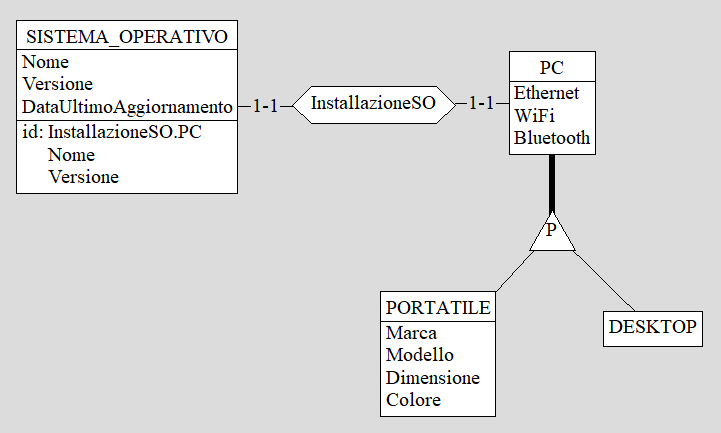
\includegraphics[width=0.6\textwidth]{images/pc.png}
    \caption{Modellazione di PC desktop e portatili e del sistema operativo installato.}
	\label{images:pc}
\end{figure}

\noindent Per le periferiche e i componenti, in base alle specifiche richieste si individuano le gerarchie di specializzazione mostrate in figura \ref{images:periferica} e \ref{images:componente}. Si evidenzia che esse hanno copertura parziale: le sotto-entità esplicitate sono le tipologie di periferiche e componenti registrate più frequentemente e/o per le quali è richiesto di riportare particolari specifiche.

\begin{figure}[H]
    \centering
	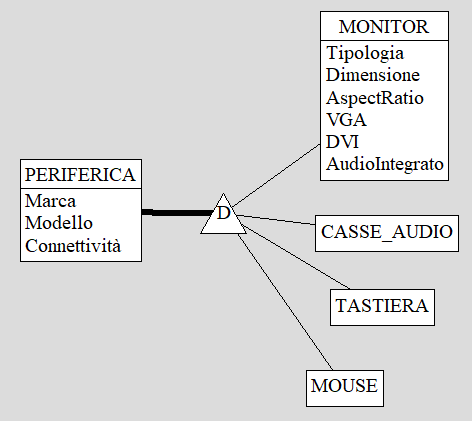
\includegraphics[width=0.6\textwidth]{images/periferica.png}
    \caption{Gerarchia delle periferiche.}
	\label{images:periferica}
\end{figure}

\begin{figure}[H]
    \centering
	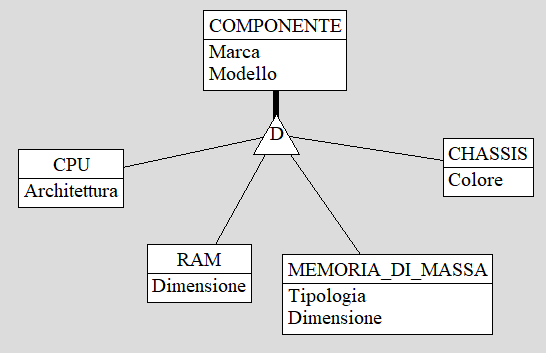
\includegraphics[width=0.6\textwidth]{images/componente.png}
    \caption{Gerarchia dei componenti.}
	\label{images:componente}
\end{figure}

\noindent Si modellano poi le associazioni tra PC e periferiche e tra PC e componenti. 
\\
I PC desktop possono essere corredati di monitor, mouse, tastiera o casse audio; si modellano quindi le associazioni opzionali tra PC desktop e tali periferiche. \\
Una periferica non deve essere necessariamente associata ad un PC, dal momento che possono essere anche ricevute/donati singolarmente.

\begin{figure}[H]
	\centering
	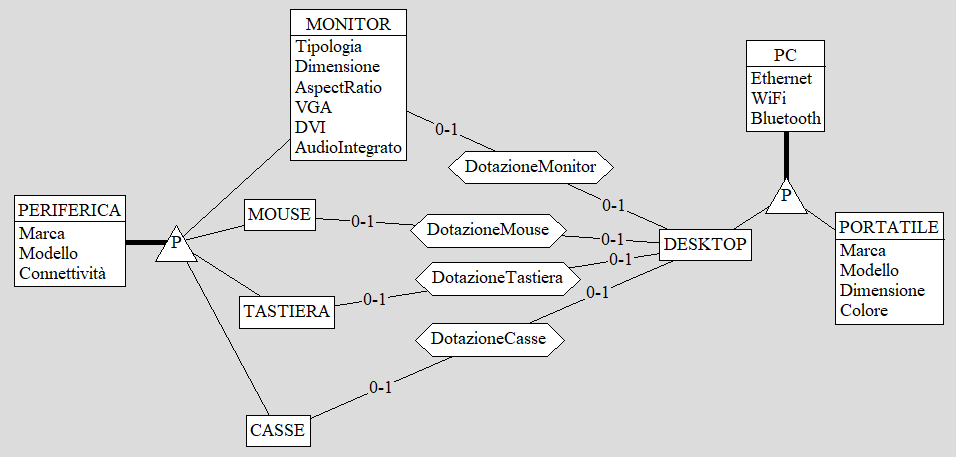
\includegraphics[width=\textwidth]{images/periferiche-pc.png}
    \caption{Associazioni tra PC e periferiche.}
	\label{images:periferiche-pc}
\end{figure}

\noindent Per quanto riguarda le componenti di ogni PC, si memorizzano quantomeno le informazioni relative alla CPU, alla RAM (possono esserne installati fino a 4 moduli), ai supporti di memoria di massa (1 o 2) e, nel caso dei PC desktop, allo chassis. Al PC possono eventualmente essere associati altri tipi di componenti, qualora ritenuto sia necessario registrarlo. \\
Un componente non deve invece essere necessariamente associato ad un PC, dal momento che possono essere anche ricevuti/donati singolarmente.

\begin{figure}[H]
	\centering
	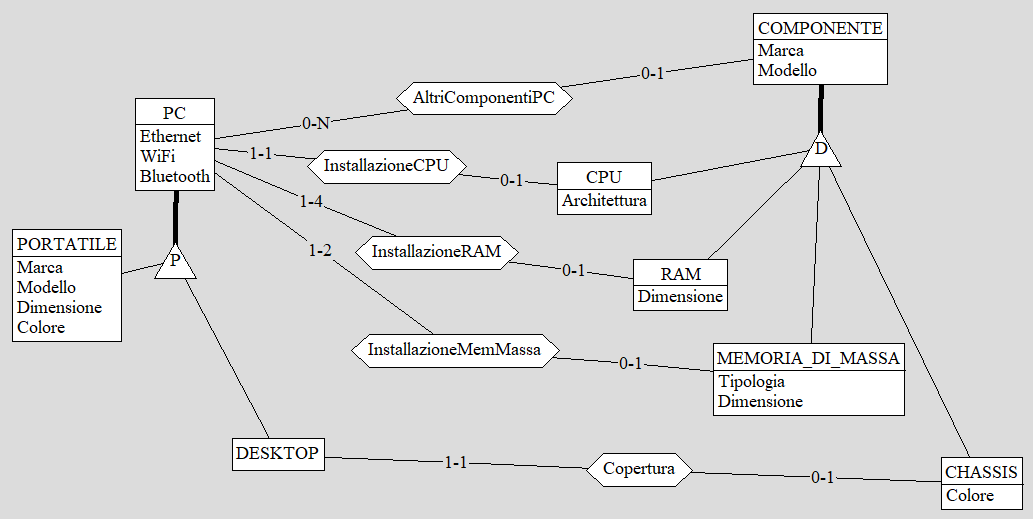
\includegraphics[width=\textwidth]{images/componenti-pc.png}
    \caption{Associazioni tra PC e componenti.}
	\label{images:componenti-pc}
\end{figure}

\section{Schema concettuale finale}

\begin{sidewaysfigure}[ht]
    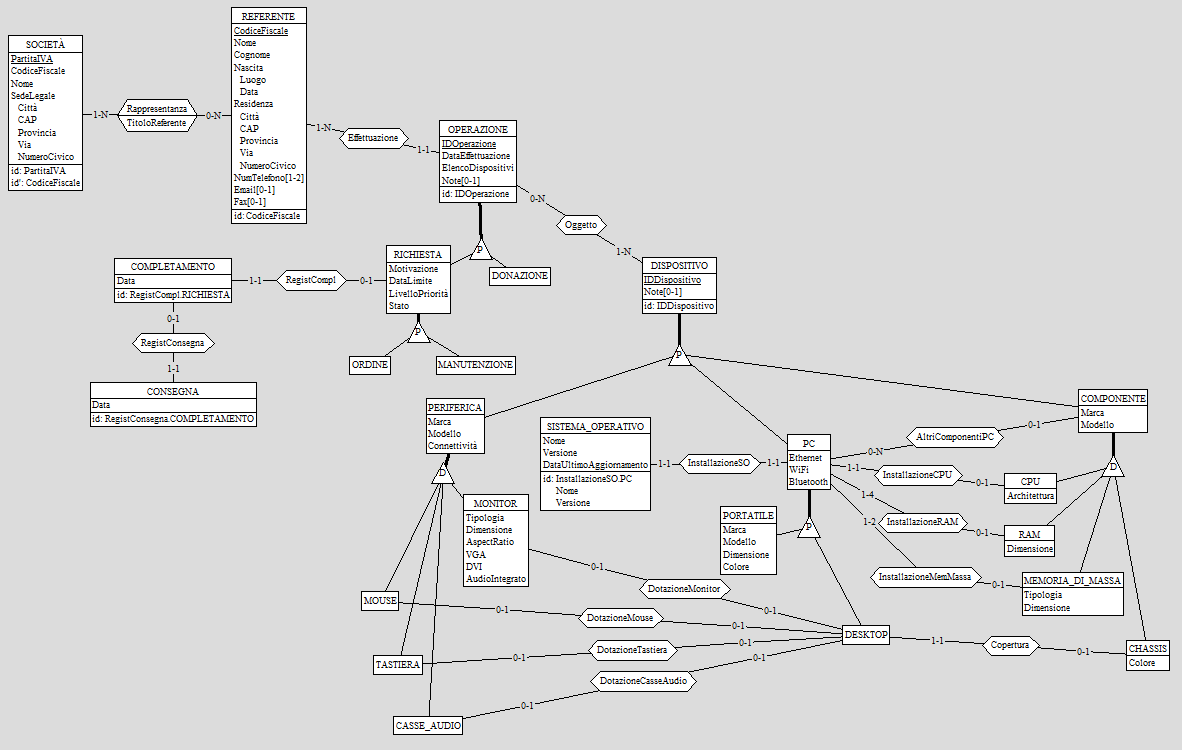
\includegraphics{images/schema-ER-completo.png}
\end{sidewaysfigure}

%------------------------------------------------------

\chapter{Progettazione logica}

\section{Stima del volume dei dati}

\newcolumntype{A}{>{\raggedright\arraybackslash}p{0.3\linewidth}}
\newcolumntype{B}{>{\raggedright\arraybackslash}p{0.2\linewidth}}
\newcolumntype{C}{>{\raggedright\arraybackslash}p{0.15\linewidth}}
\begin{table}[H]
	\begin{center}
	    	\begin{tabular}{A|C|B|A}
	      	\toprule
	      		\textbf{Concetto} & \textbf{Costrutto} & \textbf{Volume} & \textbf{Note} \\
	      	\midrule
					\hline
					Referente
					& E
					& 800
					& \\
					% ----------------------
					\hline
					Rappresentanza
					& R
					& 300
					& \\
					% ----------------------
					\hline
					Società
					& E
					& 300
					& \\
					% ----------------------
					\hline
					Effettuazione
					& R
					& 800
					& \\
					% ----------------------
					\hline
					Donazione
					& E
					& 400
					& \\
					% ----------------------
					\hline
					Ordine (Richiesta)
					& E
					& 380
					& \\
					% ----------------------
					\hline
					Manutenzione (Richiesta)
					& E
					& 20
					& \\
					% ----------------------
					\hline
					Registrazione Completamento
					& R
					& 400
					& \\
					% ----------------------
					\hline
					Completamento
					& E
					& 400
					& \\
					% ----------------------
					\hline
					Registrazione Consegna
					& R
					& 400
					& \\
					% ----------------------
					\hline
					Consegna
					& E
					& 400
					& \\
	      	\bottomrule
	    	\end{tabular}
	\end{center}
	\caption{Tabella dei volumi stimati dei dati legati all'effettuazione delle donazioni e delle richieste.}
    	\label{tab:tabella-volumi-1}
\end{table}

\newcolumntype{A}{>{\raggedright\arraybackslash}p{0.3\linewidth}}
\newcolumntype{B}{>{\raggedright\arraybackslash}p{0.15\linewidth}}
\newcolumntype{C}{>{\raggedright\arraybackslash}p{0.1\linewidth}}
\newcolumntype{D}{>{\raggedright\arraybackslash}p{0.35\linewidth}}
\begin{table}[H]
    \begin{threeparttable}
    	\begin{center}
            \begin{tabular}{A|B|C|D}
                \toprule
                    \textbf{Concetto} & \textbf{Costrutto} & \textbf{Volume} & \textbf{Note} \\
                \midrule
                        \hline
                        PC
                        & E
                        & 1200
                        & \\
                        % ----------------------
                        \hline
                        Desktop
                        & E
                        & 1000
                        & \\
                        % ----------------------
                        \hline
                        Portatile
                        & E
                        & 200
                        & \\
                        % ----------------------
                        \hline
                        Periferica
                        & E
                        & 3400
                        & \\
                        % ----------------------
                        \hline
                        Monitor
                        & E
                        & 1000
                        & \\
                        % ----------------------
                        \hline
                        Dotazione Monitor
                        & R
                        & 700
                        & Non sempre un PC desktop viene richiesto con monitor. Ciò vale anche per le altre periferiche. \\
                        % ----------------------
                        \hline
                        Tastiera
                        & E
                        & 1000
                        & \\
                        % ----------------------
                        \hline
                        Dotazione Tastiera
                        & R
                        & 700
                        & \\
                        % ----------------------
                        \hline
                        Mouse
                        & E
                        & 1000
                        & \\
                        % ----------------------
                        \hline
                        Dotazione Mouse
                        & R
                        & 700
                        & \\
                        % ----------------------
                        \hline
                        Casse Audio
                        & E
                        & 200
                        & \\
                        % ----------------------
                        \hline
                        Dotazione Casse Audio
                        & R
                        & 100
                        & Spesso i PC desktop non sono forniti insieme alle casse audio, data anche l'eventuale fornitura di un monitor con audio integrato.\\
                        % ----------------------
                        \hline
                        Componenti
                        & R
                        & 7000
                        & \\
                        % ----------------------
                        \hline
                        Chassis
                        & E
                        & 1000
                        & \\
                        % ----------------------
                        \hline
                        Copertura
                        & R
                        & 1000
                        & I PC desktop vengono sempre forniti insieme allo chassis. \\
                        % ----------------------
                        \hline
                        CPU
                        & E
                        & 1400
                        & Possono essere devoluti al Trashware anche singoli componenti, che di conseguenza possono essere più dei PC ricevuti. Ciò vale anche per ogni tipologia di singolo componente. \\
                        % ----------------------
                        \hline
                        Installazione CPU
                        & R
                        & 1200
                        & \\
                        % ----------------------
                        \hline
                        Oggetto
                        & E
                        & 17000 \tnote{1}
                        & In media, per ogni dispositivo si ha almeno un'istanza di Oggetto che lo associa alla donazione con cui è stato ricevuto. Molti dispositivi sono poi associati ad una richiesta per essere donati. \\
                \bottomrule
            \end{tabular}
            \begin{tablenotes}
                \item[1] Si supponga che 7000 siano relative a richieste e che, di queste, 800 siano relative a PC desktop e 800 siano relative a CPU.
            \end{tablenotes}
    	\end{center}
    \end{threeparttable}
\end{table}

\newcolumntype{A}{>{\raggedright\arraybackslash}p{0.3\linewidth}}
\newcolumntype{B}{>{\raggedright\arraybackslash}p{0.15\linewidth}}
\newcolumntype{C}{>{\raggedright\arraybackslash}p{0.1\linewidth}}
\newcolumntype{D}{>{\raggedright\arraybackslash}p{0.35\linewidth}}
\begin{table}[H]
	\begin{center}
	    	\begin{tabular}{A|B|C|D}
	      	\toprule
	      		\textbf{Concetto} & \textbf{Costrutto} & \textbf{Volume} & \textbf{Note} \\
	      	\midrule
					\hline
					RAM
					& E
					& 2700
					& \\
					% ----------------------
					\hline
					Installazione RAM
					& R
					& 2500
					& Solitamente si installano 2 banchi di RAM per PC (desktop o portatile), talvolta più di 2. \\
					% ----------------------
					\hline
					Memoria di massa
					& E
					& 1500
					& \\
					% ----------------------
					\hline
					InstallazioneMemMassa
					& R
					& 1300
					& Tavolta, su un PC si installano due supporti di memoria (es. un HDD e un SSD). \\
					% ----------------------
					\hline
					AltriComponentiPC
					& R
					& 300
					& Se considerato utile, vengono registrate informazioni anche su altri componenti di un PC oltre a quelle già citate.\\
					% ----------------------
					\hline
					Sistema Operativo
					& E
					& 1200
					& \\
					% ----------------------
					\hline
					Installazione SO
					& R
					& 1200
					& \\
	      	\bottomrule
	    	\end{tabular}
	\end{center}
	\caption{Tabella dei volumi stimati dei dati legati ai dispositivi.}
    	\label{tab:tabella-volumi}
\end{table}

\section{Descrizione e frequenza delle operazioni principali}

Le operazioni principali effettuate sono quelle precedentemente elencate nella sottosezione \ref{Operazioni} al momento dell'esposizione dei requisiti. Vengono qui riproposte, indicandone anche la frequenza stimata.

\newcolumntype{A}{>{\raggedright\arraybackslash}p{0.5\linewidth}}
\newcolumntype{B}{>{\raggedright\arraybackslash}p{0.3\linewidth}}
\newcolumntype{C}{>{\raggedright\arraybackslash}p{0.15\linewidth}}
\begin{table}[H]
	\begin{center}
	    	\begin{tabular}{C|A|B}
	      	\toprule
	      		\textbf{Codice Op.} & \textbf{Operazione} & \textbf{Frequenza} \\
	      	\midrule
					\hline
					1
					& Registrazione di una nuova operazione
					& 5 a settimana \\
					% ----------------------
					\hline
					2
					& Visualizzazione delle donazioni ricevute dal progetto
					& 2 al giorno \\
                    % ----------------------
					\hline
					3
					& Visualizzazione delle richieste ricevute, divise per stato corrente e in ordine decrescente di priorità
					& 5 al giorno \\
                    % ----------------------
					\hline
					4
					& Aggiornamento dello stato di lavorazione di una richiesta (registrazione del suo completamento e della sua consegna)
					& 4 a settimana (si supponga che 2 siano completamenti e 2 siano consegne) \\
					% ----------------------
					\hline
					5
					& Inserimento di un nuovo dispositivo in inventario
					& 80 a settimana (si supponga che si registrino 10 PC desktop, 2 PC portatili, 50 componenti e 18 periferiche) \\
					% ----------------------
					\hline
					6
					& Visualizzazione delle informazioni sui dispositivi registrati in inventario, filtrando per tipologia di dispositivo
					& 30 al giorno (si supponga che 10 siano per PC desktop, 10 per monitor e 5 per CPU) \\
                    % ----------------------
					\hline
					7
					& Associazione di un dispositivo ad un'operazione
					& 10 al giorno \\
                     % ----------------------
					\hline
					8
					& Associazione di un componente ad un PC o di una periferica ad un PC desktop
					& 10 al giorno \\
	      	\bottomrule
	    	\end{tabular}
	\end{center}
	\caption{Frequenza delle operazioni principali.}
    	\label{tab:tabella-frequenze}
\end{table}

\section{Schemi di navigazione e tabelle degli accessi}

Di seguito, vengono mostrate le tabelle degli accessi per ogni operazione principale, le quali riportano il numero stimato di accessi in lettura e in scrittura su entità e associazioni in base alla frequenza stimata dell'operazione. \\
Lo schema di navigazione viene riportato per le operazioni il cui cammino logico non è di immediata comprensione. \\
Si evidenzia che, nel calcolo dei costi delle operazioni, gli accessi in scrittura hanno peso doppio rispetto agli accessi in lettura.

\subsubsection{Op. 1: registrazione di una nuova operazione}

L'operazione comporta anche le registrazione dei dati relativi al referente ed eventualmente alla società che rappresenta. Si ha quindi la creazione non solo di un'istanza di Donazione o Richiesta, ma anche la creazione di un'istanza dell'entità Referente e dell'associazione Effettuazione, ed eventualmente anche di un'istanza dell'entità Società e dell'associazione Rappresentanza.
Può anche accadere che un cliente e una società siano già registrati, ma è un'eventualità che si verifica poco frequentemente, che si può non considerare nel calcolo del costo medio.

\newcolumntype{A}{>{\raggedright\arraybackslash}p{0.3\linewidth}}
\newcolumntype{B}{>{\raggedright\arraybackslash}p{0.15\linewidth}}
\newcolumntype{C}{>{\centering\arraybackslash}p{\linewidth}}
\begin{table}[H]
	\begin{center}
	    \begin{tabular}{A|B|A|B}
	      	\toprule
	      		\textbf{Concetto} & \textbf{Costrutto} & \textbf{Accessi} & \textbf{Tipo} \\
	      	\midrule
				\hline
				Referente
				& E
				& 1
				& S \\
				% ----------------------
				\hline
				Rappresentanza
				& R
				& 300 / 800 = 0.375
				& S \\
				% ----------------------
				\hline
				Società
				& E
				& 300 / 800 = 0.375
				& S \\
				% ----------------------
				\hline
				Effettuazione
				& R
				& 1
				& S \\
				% ----------------------
				\hline
				Donazione / Richiesta
				& E
				& 1
				& S \\
	      	\bottomrule
                \multicolumn{4}{|C|}{Totale: 3.75 S $\xrightarrow{}$ Costo = $3.75 \times 2 \times 5$ a settimana = 37.5 a settimana}
	    \end{tabular}
	\end{center}
\end{table}

\subsubsection{Op. 2: visualizzazione delle donazioni
ricevute dal progetto}

La visualizzazione delle informazioni relative alle donazioni implica anche l'accesso alle informazioni sui referenti e sull'eventuale società di cui è rappresentante.

\noindent Secondo le stime effettuate, le donazioni sono la metà delle operazioni totali registrate; per questo motivo, si considerano volumi dimezzati anche per quanto riguarda gli accessi relativi a referenti e società.

\newcolumntype{A}{>{\raggedright\arraybackslash}p{0.3\linewidth}}
\newcolumntype{B}{>{\raggedright\arraybackslash}p{0.15\linewidth}}
\newcolumntype{C}{>{\centering\arraybackslash}p{\linewidth}}
\begin{table}[H]
	\begin{center}
	    \begin{tabular}{A|B|A|B}
	      	\toprule
	      		\textbf{Concetto} & \textbf{Costrutto} & \textbf{Accessi} & \textbf{Tipo} \\
	      	\midrule
				\hline
				Donazione
				& E
				& 400
				& L \\
                % ----------------------
				\hline
				Effettuazione
				& R
				& 800 / 2 = 400
				& L \\
                % ----------------------
				\hline
				Referente
				& E
				& 800 / 2 = 400
				& L \\
				% ----------------------
				\hline
				Rappresentanza
				& R
				& 300 / 2 = 150
				& L \\
				% ----------------------
				\hline
				Società
				& E
				& 300 / 2 = 150
				& L \\
	      	\bottomrule
                \multicolumn{4}{|C|}{Totale: 1500 L $\xrightarrow{}$ Costo = $1500 \times 2$ al giorno = 3000 al giorno}
	    \end{tabular}
	\end{center}
\end{table}

\begin{figure}[H]
	\centering
	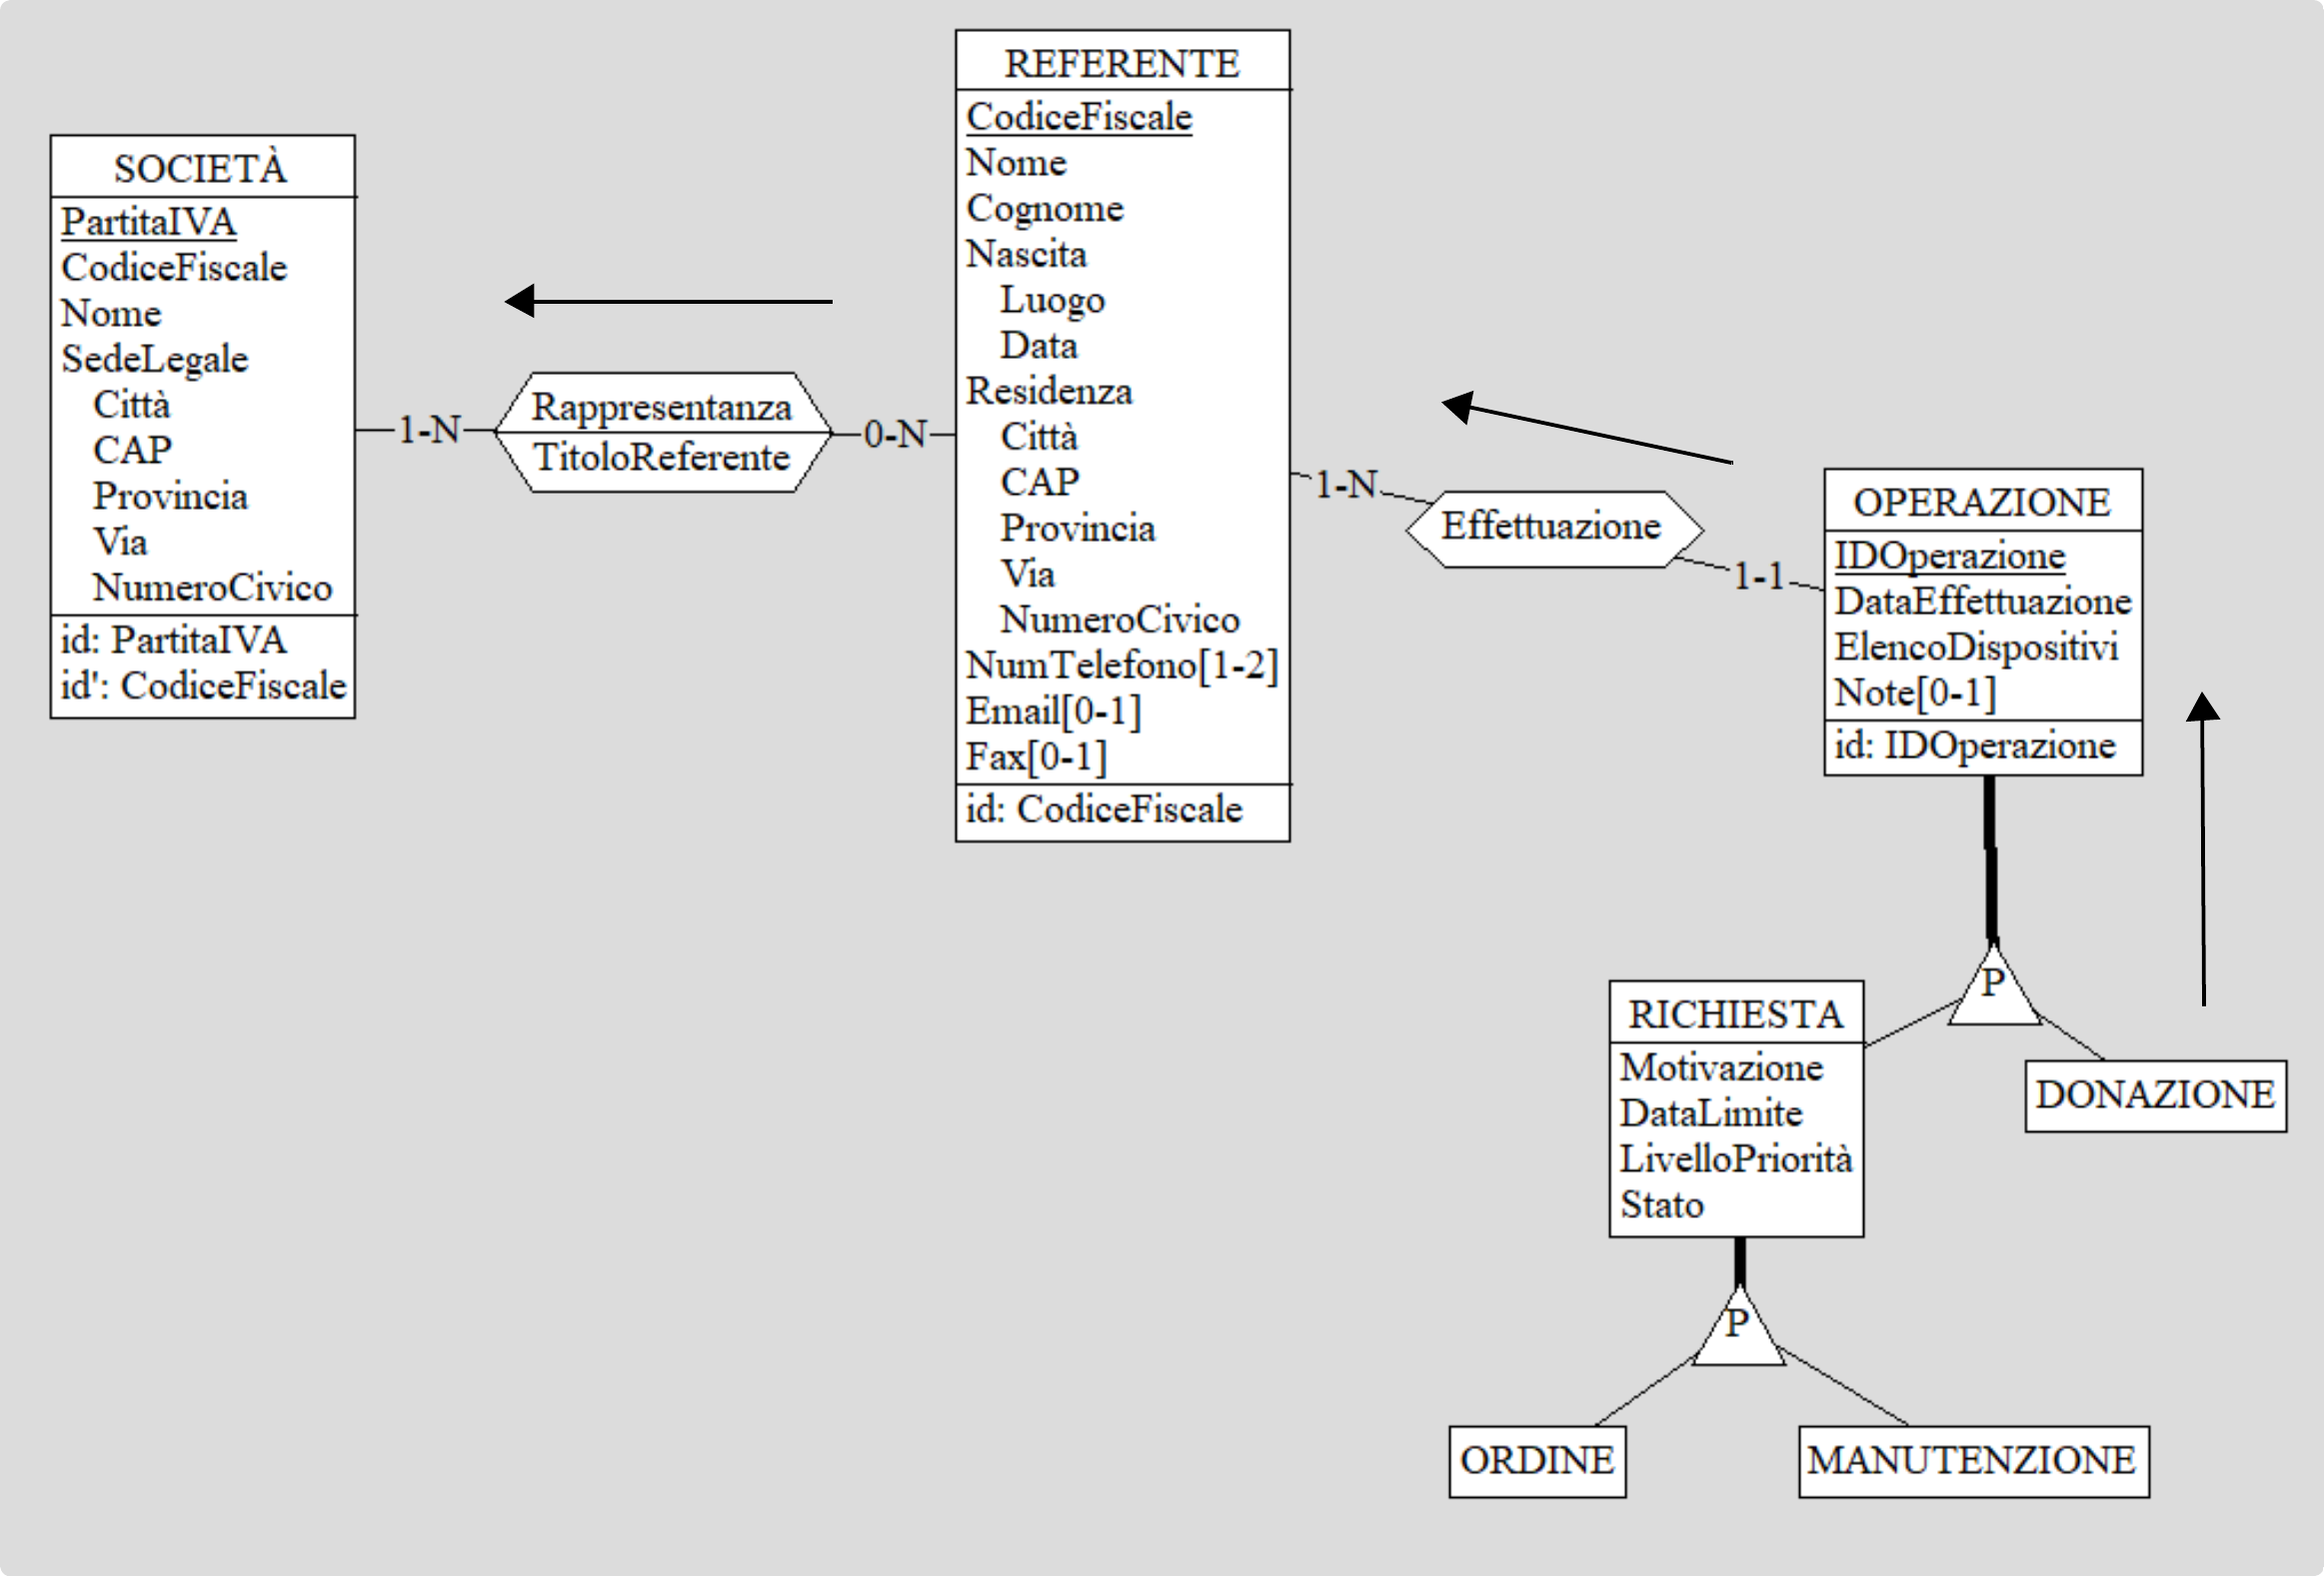
\includegraphics[width=\textwidth]{images/nav-op2.png}
\end{figure}

\subsubsection{Op. 3: visualizzazione delle richieste
ricevute, divise per stato corrente e in
ordine decrescente di priorità}

La visualizzazione delle richieste comporta gli accessi alle stesse entità e associazioni interessate dalla visualizzazione delle donazioni. La divisione per stato corrente e l'ordinamento di priorità non comportano altri accessi, dato che si basano su attributi della Richiesta.

Analogamente all'operazione 2, le richieste sono la metà delle operazioni totali registrate; per questo motivo, si considerano volumi dimezzati anche per quanto riguarda gli accessi relativi a referenti e società.

\newcolumntype{A}{>{\raggedright\arraybackslash}p{0.3\linewidth}}
\newcolumntype{B}{>{\raggedright\arraybackslash}p{0.15\linewidth}}
\newcolumntype{C}{>{\centering\arraybackslash}p{\linewidth}}
\begin{table}[H]
	\begin{center}
	    \begin{tabular}{A|B|A|B}
	      	\toprule
	      		\textbf{Concetto} & \textbf{Costrutto} & \textbf{Accessi} & \textbf{Tipo} \\
	      	\midrule
				\hline
				Richiesta
				& E
				& 400
				& L \\
                % ----------------------
				\hline
				Effettuazione
				& R
				& 800 / 2 = 400
				& L \\
                % ----------------------
				\hline
				Referente
				& E
				& 800 / 2 = 400
				& L \\
				% ----------------------
				\hline
				Rappresentanza
				& R
				& 300 / 2 = 150
				& L \\
				% ----------------------
				\hline
				Società
				& E
				& 300 / 2 = 150
				& L \\
	      	\bottomrule
                \multicolumn{4}{|C|}{Totale: 1500 L $\xrightarrow{}$ Costo = $1500 \times 5$ al giorno = 7500 al giorno}
	    \end{tabular}
	\end{center}
\end{table}

\begin{figure}[H]
	\centering
	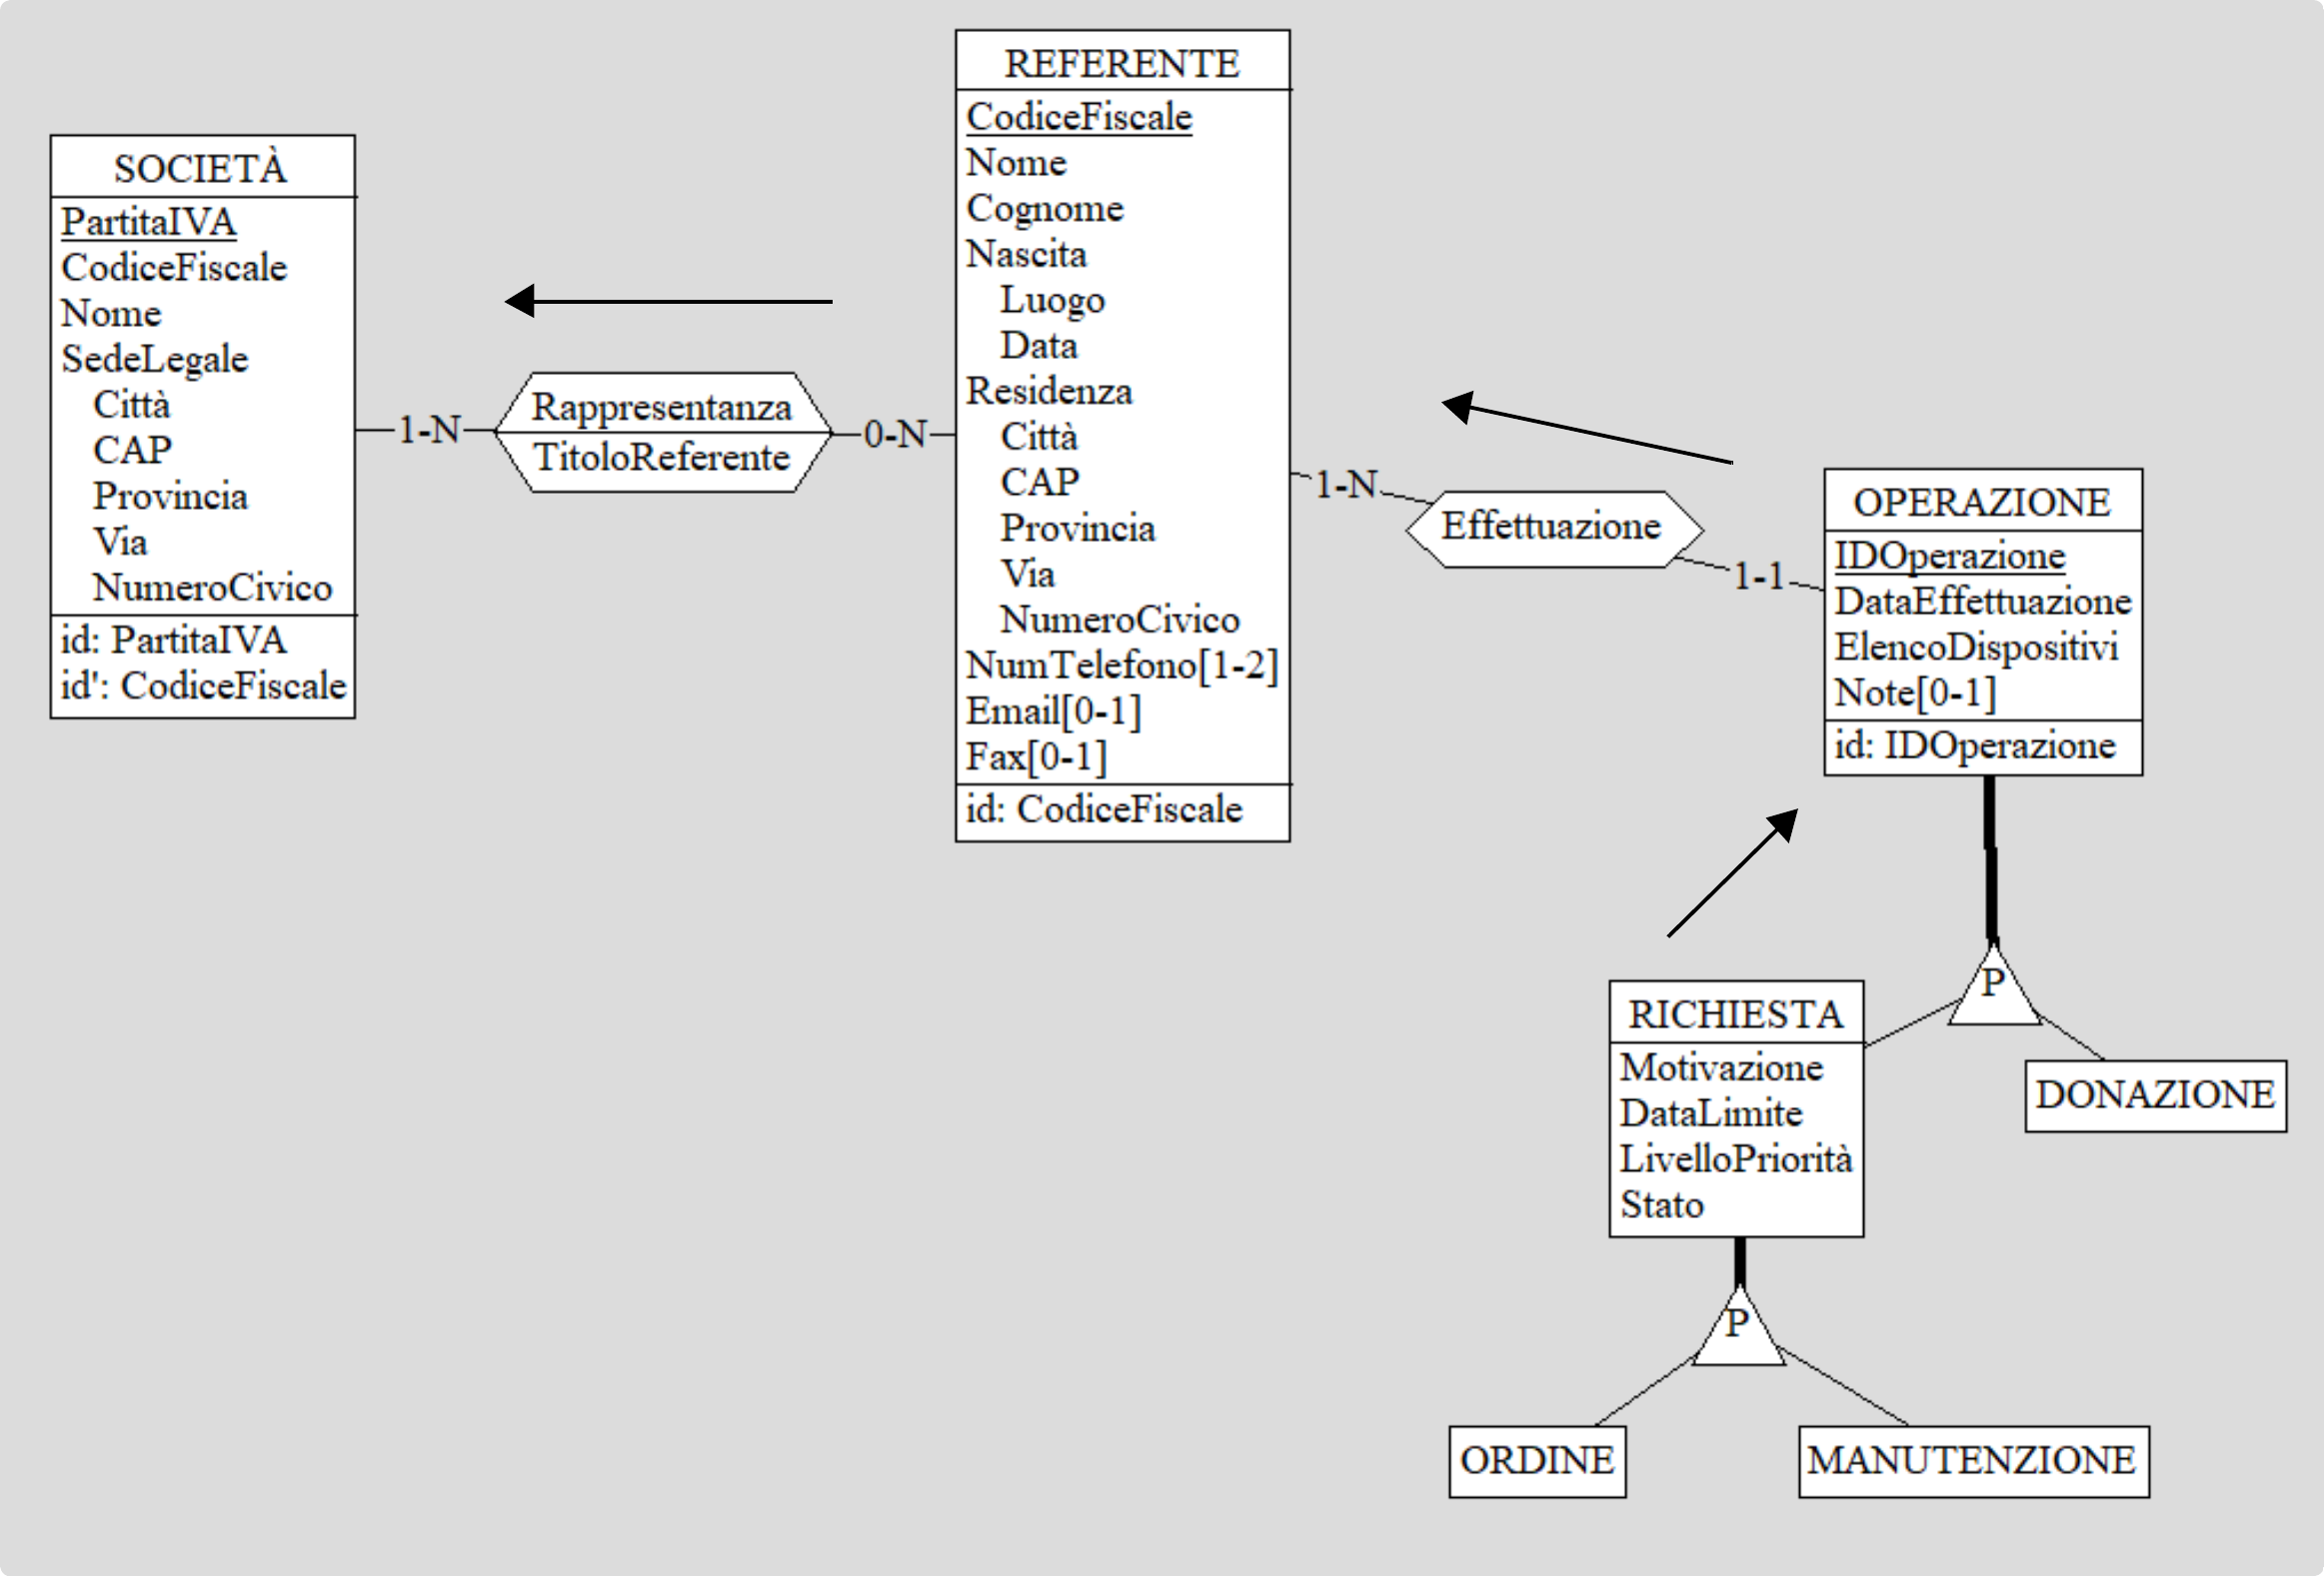
\includegraphics[width=\textwidth]{images/nav-op3.png}
\end{figure}

\noindent Per la visualizzazione delle date di completamento e di consegna, sono necessari altri accessi.

\newcolumntype{A}{>{\raggedright\arraybackslash}p{0.3\linewidth}}
\newcolumntype{B}{>{\raggedright\arraybackslash}p{0.15\linewidth}}
\newcolumntype{C}{>{\centering\arraybackslash}p{\linewidth}}
\begin{table}[H]
	\begin{center}
	    \begin{tabular}{A|B|A|B}
	      	\toprule
	      		\textbf{Concetto} & \textbf{Costrutto} & \textbf{Accessi} & \textbf{Tipo} \\
	      	\midrule
				\hline
				Regist. Completamento
				& E
				& 400
				& L \\
                % ----------------------
				\hline
				Completamento
				& R
				& 400
				& L \\
	      	\bottomrule
                \multicolumn{4}{|C|}{Totale: 800 L $\xrightarrow{}$ Costo = $800 \times 5$ al giorno = 4000 al giorno}
	    \end{tabular}
	\end{center}
\end{table}

\newcolumntype{A}{>{\raggedright\arraybackslash}p{0.3\linewidth}}
\newcolumntype{B}{>{\raggedright\arraybackslash}p{0.15\linewidth}}
\newcolumntype{C}{>{\centering\arraybackslash}p{\linewidth}}
\begin{table}[H]
	\begin{center}
	    \begin{tabular}{A|B|A|B}
	      	\toprule
	      		\textbf{Concetto} & \textbf{Costrutto} & \textbf{Accessi} & \textbf{Tipo} \\
	      	\midrule
				\hline
				Regist. Consegna
				& E
				& 400
				& L \\
                % ----------------------
				\hline
				Consegna
				& R
				& 400
				& L \\
	      	\bottomrule
                \multicolumn{4}{|C|}{Totale: 800 L $\xrightarrow{}$ Costo = $800 \times 5$ al giorno = 4000 al giorno}
	    \end{tabular}
	\end{center}
\end{table}

\noindent Si ha quindi un costo totale giornaliero di $7500 + 4000 + 4000 = 15500$.

\subsubsection{Op.4: aggiornamento dello stato di
lavorazione di una richiesta (registrazione del suo completamento
e della sua consegna)}

Per quanto riguarda la registrazione del completamento di una consegna, si hanno i seguenti accessi. Supponendo di conoscere il codice associato alla richiesta di cui deve essere aggiornato lo stato, si ha una lettura della Richiesta cercata e una scrittura su di essa per aggiornare l'attributo relativo allo stato; si ha poi una creazione di un'istanza di Completamento legata alla Richiesta.

\newcolumntype{A}{>{\raggedright\arraybackslash}p{0.3\linewidth}}
\newcolumntype{B}{>{\raggedright\arraybackslash}p{0.15\linewidth}}
\newcolumntype{C}{>{\centering\arraybackslash}p{\linewidth}}
\begin{table}[H]
	\begin{center}
	    \begin{tabular}{A|B|A|B}
	      	\toprule
	      		\textbf{Concetto} & \textbf{Costrutto} & \textbf{Accessi} & \textbf{Tipo} \\
	      	\midrule
				\hline
				Richiesta
				& E
				& 1
				& L \\
                % ----------------------
                \hline
				Richiesta
				& E
				& 1
				& S \\
                % ----------------------
                \hline
				Regist. Completamento
				& R
				& 1
				& S \\
                % ----------------------
                \hline
				Completamento
				& E
				& 1
				& S \\
                % ----------------------
	      	\bottomrule
                \multicolumn{4}{|C|}{Totale: 1L + 3S  $\xrightarrow{}$ Costo = $(1 + 3 \times 2) \times 2$ a settimana = 14 a settimana}
	    \end{tabular}
	\end{center}
\end{table}

\noindent Per quanto riguarda la registrazione delle consegne, oltre alla lettura e scrittura su Richiesta, è necessario leggere il Completamento associato alla Richiesta, al quale viene poi associata la nuova istanza di Consegna che viene creata.

\newcolumntype{A}{>{\raggedright\arraybackslash}p{0.3\linewidth}}
\newcolumntype{B}{>{\raggedright\arraybackslash}p{0.15\linewidth}}
\newcolumntype{C}{>{\centering\arraybackslash}p{\linewidth}}
\begin{table}[H]
	\begin{center}
	    \begin{tabular}{A|B|A|B}
	      	\toprule
	      		\textbf{Concetto} & \textbf{Costrutto} & \textbf{Accessi} & \textbf{Tipo} \\
	      	\midrule
				\hline
				Richiesta
				& E
				& 1
				& L \\
                % ----------------------
                \hline
				Richiesta
				& E
				& 1
				& S \\
                % ----------------------
                \hline
				Regist. Completamento
				& R
				& 1
				& L \\
                % ----------------------
                \hline
				Completamento
				& E
				& 1
				& L \\
                % ----------------------
                \hline
				Regist. Consegna
				& R
				& 1
				& S \\
                % ----------------------
                \hline
				Consegna
				& E
				& 1
				& S \\
	      	\bottomrule
                \multicolumn{4}{|C|}{Totale: 3L + 3S  $\xrightarrow{}$ Costo = $(3 + 3 \times 2) \times 2$ a settimana = 18 a settimana}
	    \end{tabular}
	\end{center}
\end{table}

\subsubsection{Op. 5: inserimento di un nuovo dispositivo in
inventario}

L'inserimento di una nuova periferica o di un nuovo componente è banale: richiede solo la creazione di una nuova istanza di periferica/componente, sia essa una delle specializzazione esplicitate nello schema oppure un altro tipo di periferica/componente rappresentato da una generica istanza di Periferica/Componente. \\ 
Secondo le stime, si registrano 50 componenti e 18 periferiche al giorno, avendo così 68 scritture per un costo giornaliero di $68 \times 2 = 136$.

\noindent Più complessa è invece la registrazione di un PC. \\
Per quanto riguarda un PC portatile, oltre alla creazione di un'istanza di PC Portatile, si ha anche la creazione di un'istanza di Sistema Operativo e delle associazioni che lo legano ai suoi componenti (i quali vanno registrati prima).
In media, ad un PC si associano una CPU, 2 moduli di RAM e 1 dispositivo di memoria di massa.

\newcolumntype{A}{>{\raggedright\arraybackslash}p{0.3\linewidth}}
\newcolumntype{B}{>{\raggedright\arraybackslash}p{0.15\linewidth}}
\newcolumntype{C}{>{\centering\arraybackslash}p{\linewidth}}
\begin{table}[H]
	\begin{center}
	    \begin{tabular}{A|B|A|B}
	      	\toprule
	      		\textbf{Concetto} & \textbf{Costrutto} & \textbf{Accessi} & \textbf{Tipo} \\
	      	\midrule
				\hline
				Portatile
				& E
				& 1
				& S \\
                % ----------------------
                \hline
				Installazione SO
				& E
				& 1
				& S \\
                % ----------------------
                \hline
				Sistema Operativo
				& E
				& 1
				& S \\
                % ----------------------
                \hline
				Installazione CPU
				& R
				& 1
				& S \\
                % ----------------------
                \hline
				Installazione RAM
				& R
				& 2
				& S \\
                % ----------------------
                \hline
				Installazione Mem. Massa
				& R
				& 1
				& S \\
	      	\bottomrule
                \multicolumn{4}{|C|}{Totale: 7S $\xrightarrow{}$ Costo = $7 \times 2 \times 2$ a settimana = 28 a settimana}
	    \end{tabular}
	\end{center}
\end{table}

\noindent La registrazione di un PC desktop richiede anche di registrare l'associazione che lo lega al suo chassis ed eventualmente anche le associazioni con periferiche.

\newcolumntype{A}{>{\raggedright\arraybackslash}p{0.3\linewidth}}
\newcolumntype{B}{>{\raggedright\arraybackslash}p{0.15\linewidth}}
\newcolumntype{C}{>{\centering\arraybackslash}p{\linewidth}}
\begin{table}[H]
	\begin{center}
	    \begin{tabular}{A|B|A|B}
	      	\toprule
	      		\textbf{Concetto} & \textbf{Costrutto} & \textbf{Accessi} & \textbf{Tipo} \\
	      	\midrule
				\hline
				Desktop
				& E
				& 1
				& S \\
                % ----------------------
                \hline
				Installazione SO
				& E
				& 1
				& S \\
                % ----------------------
                \hline
				Sistema Operativo
				& E
				& 1
				& S \\
                % ----------------------
                \hline
				Installazione CPU
				& R
				& 1
				& S \\
                % ----------------------
                \hline
				Installazione RAM
				& R
				& 2
				& S \\
                % ----------------------
                \hline
				Installazione Mem. Massa
				& R
				& 1
				& S \\
                % ----------------------
                \hline
				Copertura
				& R
				& 1
				& S \\
                % ----------------------
                \hline
				Dotazione Monitor
				& R
				& 700 / 1000 = 0.7
				& S \\
                % ----------------------
                \hline
				Dotazione Tastiera
				& R
				& 700 / 1000 = 0.7
				& S \\
                % ----------------------
                \hline
				Dotazione Mouse
				& R
				& 700 / 1000 = 0.7
				& S \\
                % ----------------------
                \hline
				Dotazione Casse Audio
				& R
				& 100 / 1000 = 0.1
				& S \\
	      	\bottomrule
                \multicolumn{4}{|C|}{Totale: 10.2 S $\xrightarrow{}$ Costo = $10.2 \times 2 \times 10$ a settimana = 204 a settimana}
	    \end{tabular}
	\end{center}
\end{table}

\subsubsection{Op. 6: visualizzazione delle informazioni legate ai dispositivi in inventario, filtrando per tipologia di dispositivo}

Per quanto riguarda i componenti, oltre alle informazioni sui singoli componenti, risulta utile visualizzare anche l'identificativo del PC e della richiesta a cui potrebbero essere legati. \\
Nel caso delle CPU, ad esempio, si hanno i seguenti accessi.

\newcolumntype{A}{>{\raggedright\arraybackslash}p{0.3\linewidth}}
\newcolumntype{B}{>{\raggedright\arraybackslash}p{0.15\linewidth}}
\newcolumntype{C}{>{\centering\arraybackslash}p{\linewidth}}
\begin{table}[H]
	\begin{center}
	    \begin{tabular}{A|B|A|B}
	      	\toprule
	      		\textbf{Concetto} & \textbf{Costrutto} & \textbf{Accessi} & \textbf{Tipo} \\
	      	\midrule
				\hline
				CPU
				& E
				& 1400
				& L \\
                % ----------------------
                \hline
                Installazione CPU
                & R
				& 1200
				& L \\
                % ----------------------
                \hline
                Oggetto
                & R
				& 800
				& L \\
                % ----------------------
                \hline
                Richiesta
                & R
				& 800
				& L \\
	      	\bottomrule
                \multicolumn{4}{|C|}{Totale: 4200 L $\xrightarrow{}$ Costo = $4200 \times 5$ al giorno = 21000}
	    \end{tabular}
	\end{center}
    \label{tab:tabella-accessi-op6}
\end{table}

Gli accessi da svolgere sono analoghi per la altre tipologie di componenti e per le tipologie di periferiche che possono essere associate ad un PC desktop.

La visualizzazione delle informazioni legate ai PC è invece più complessa, dato che richiede di accedere anche alle informazioni sul sistema operativo installato e sui suoi componenti e di ottenere gli identificativi delle eventuali periferiche associate (se è un PC desktop).

\newcolumntype{A}{>{\raggedright\arraybackslash}p{0.3\linewidth}}
\newcolumntype{B}{>{\raggedright\arraybackslash}p{0.15\linewidth}}
\newcolumntype{C}{>{\centering\arraybackslash}p{\linewidth}}
\begin{table}[H]
	\begin{center}
	    \begin{tabular}{A|B|A|B}
	      	\toprule
	      		\textbf{Concetto} & \textbf{Costrutto} & \textbf{Accessi} & \textbf{Tipo} \\
	      	\midrule
				\hline
				Desktop
				& E
				& 1000
				& L \\
                % ----------------------
                \hline
                Installazione CPU
                & R
				& 1000
				& L \\
                % ----------------------
                \hline
                CPU
                & E
				& 1000
				& L \\
                % ----------------------
                \hline
                Installazione RAM
                & R
				& 2000
				& L \\
                % ----------------------
                \hline
                RAM
                & E
				& 2000
				& L \\
                % ----------------------
                \hline
                Installazione Mem. Massa
                & R
				& 1500
				& L \\
                % ----------------------
                \hline
                Memoria Di Massa
                & E
				& 1500
				& L \\
                % ----------------------
                \hline
                Copertura
                & R
				& 1000
				& L \\
                % ----------------------
                \hline
                Chassis
                & E
				& 1000
				& L \\
                % ----------------------
                \hline
                Dotazione Monitor
                & R
				& 700
				& L \\
                % ----------------------
                \hline
                Monitor
                & E
				& 700
				& L \\
                % ----------------------
                \hline
                Dotazione Tastiera
                & R
				& 700
				& L \\
                % ----------------------
                \hline
                Tastiera
                & E
				& 700
				& L \\
                % ----------------------
                \hline
                Dotazione Mouse
                & R
				& 700
				& L \\
                % ----------------------
                \hline
                Mouse
                & E
				& 700
				& L \\
                % ----------------------
                \hline
                Dotazione Casse Audio
                & R
				& 100
				& L \\
                % ----------------------
                \hline
                Casse Audio
                & E
				& 100
				& L \\
                % ----------------------
                \hline
                Oggetto
                & R
				& 800
				& L \\
                % ----------------------
                \hline
                Richiesta
                & R
				& 800
				& L \\
	      	\bottomrule
                \multicolumn{4}{|C|}{Totale: 18000 L $\xrightarrow{}$ Costo = $ 18000 \times 10 $ al giorno = 180000 al giorno}
	    \end{tabular}
	\end{center}
    \label{tab:tabella-accessi-op6}
\end{table}

\begin{figure}[H]
	\centering
	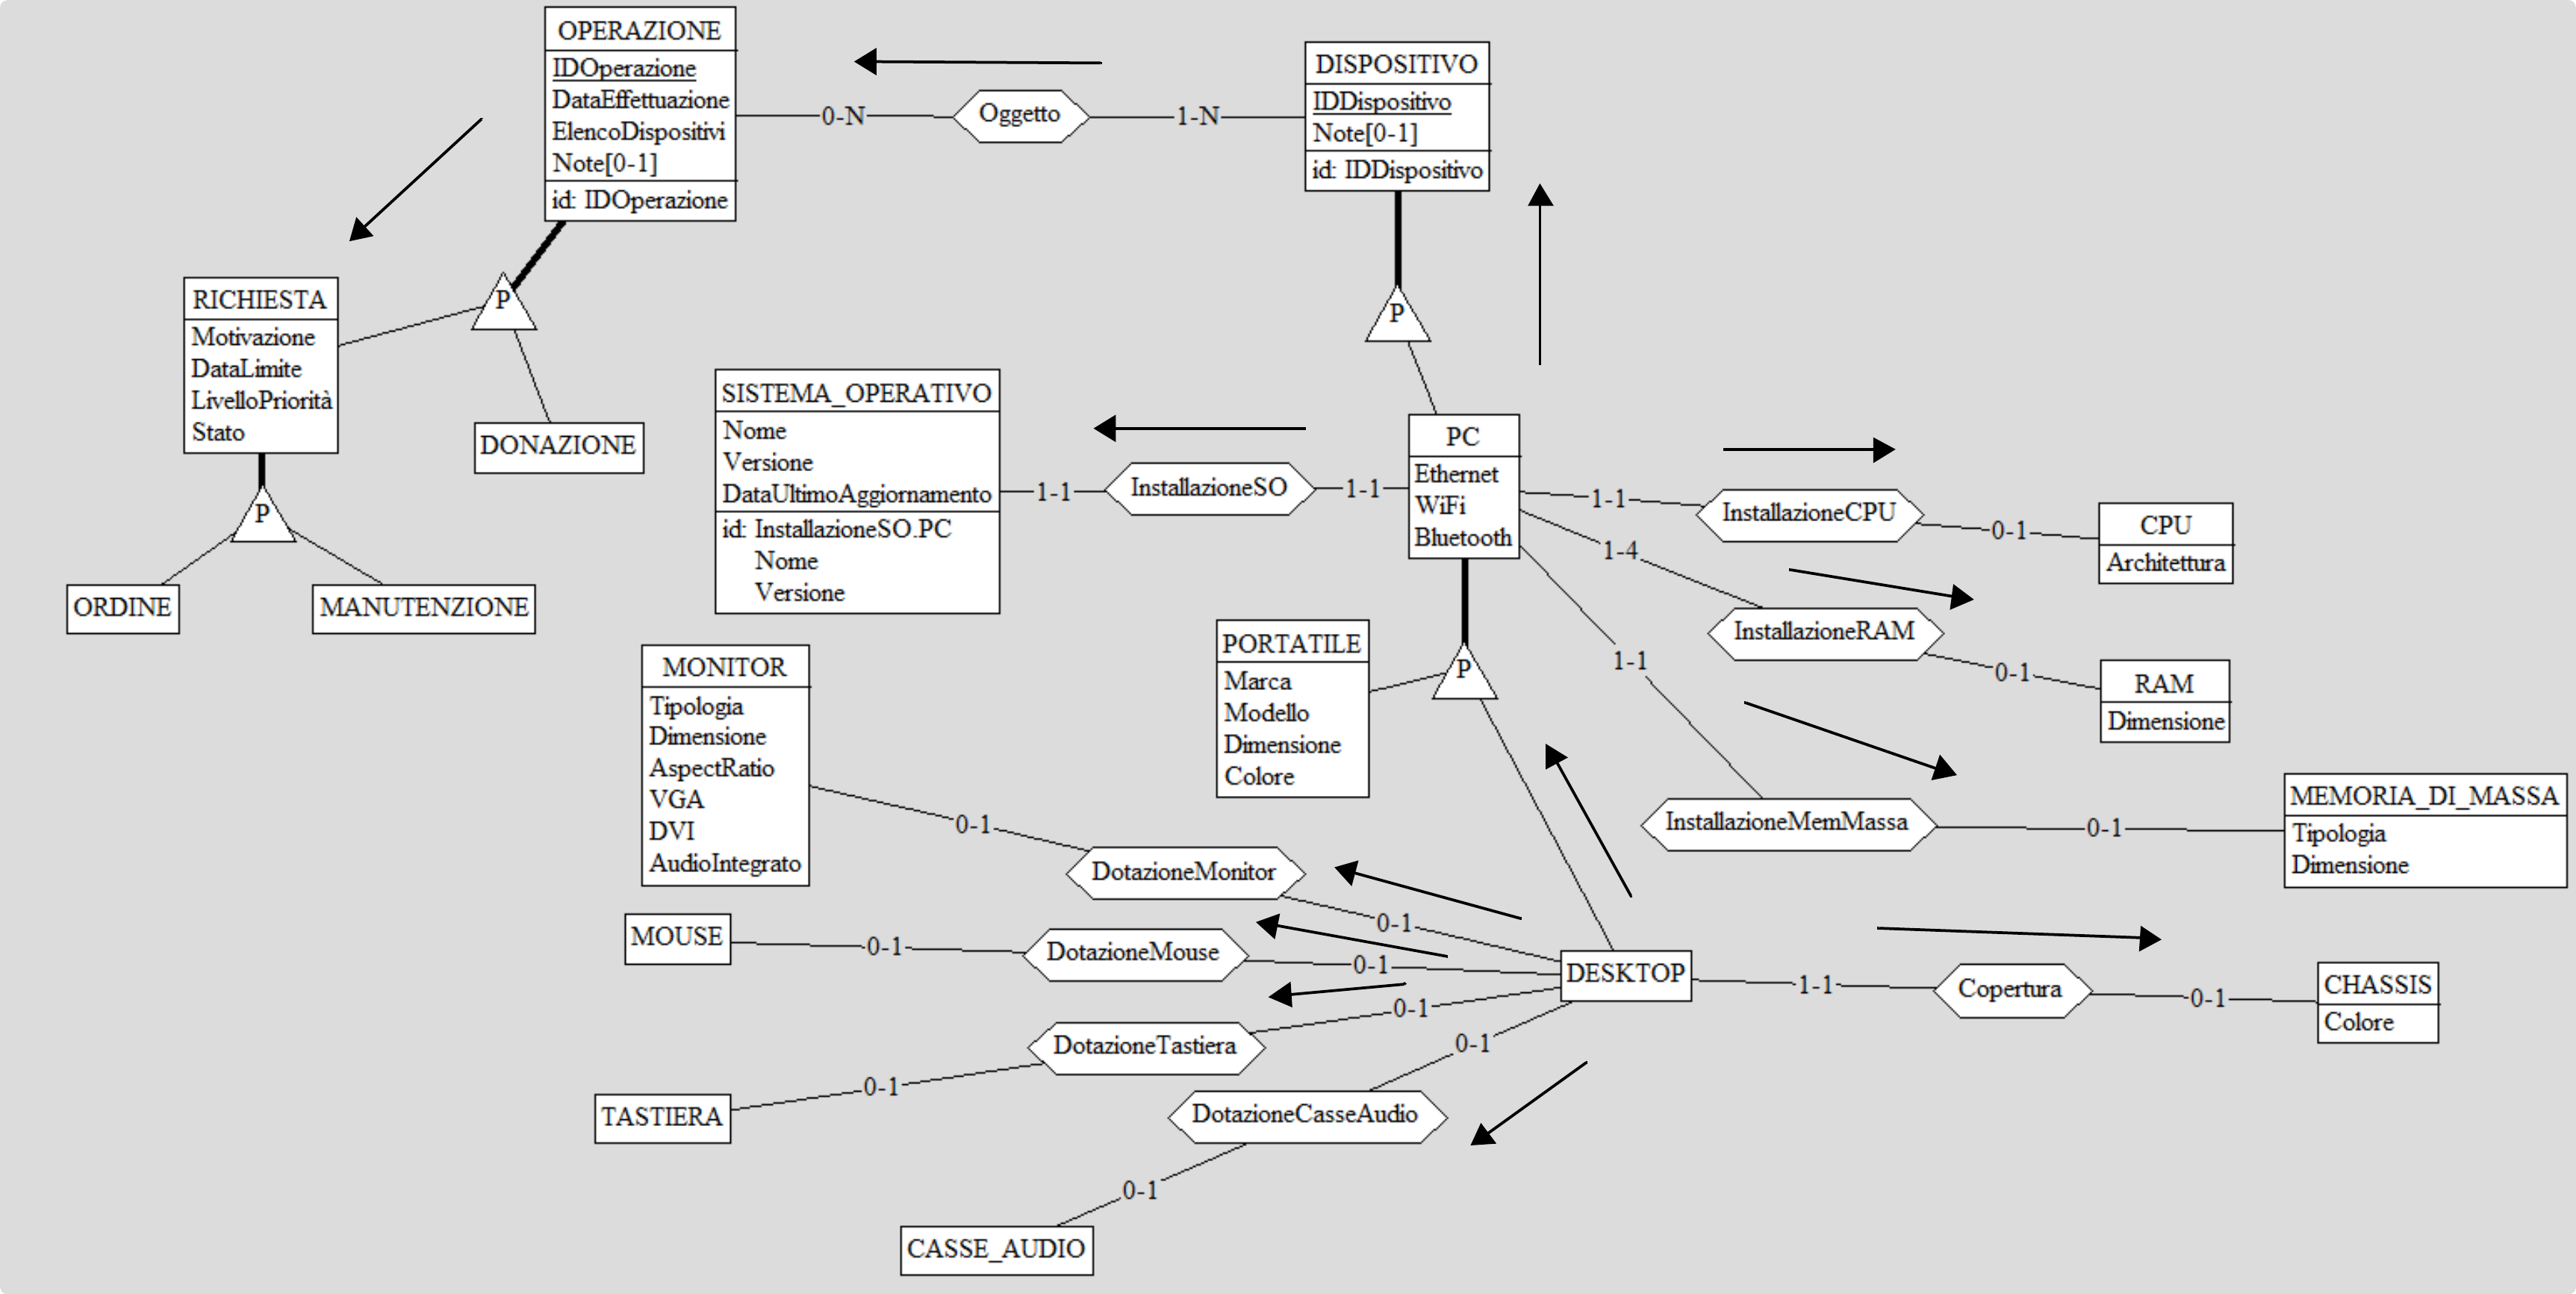
\includegraphics[width=\textwidth]{images/nav-op6.png}
\end{figure}

\subsubsection{Op. 7: associazione di un dispositivo ad un’operazione}

Dati gli identificativi di un dispositivo e di un'operazione, per associare il dispositivo all'operazione è sufficiente creare un'istanza dell'associazione Oggetto.

\newcolumntype{A}{>{\raggedright\arraybackslash}p{0.3\linewidth}}
\newcolumntype{B}{>{\raggedright\arraybackslash}p{0.15\linewidth}}
\newcolumntype{C}{>{\centering\arraybackslash}p{\linewidth}}
\begin{table}[H]
	\begin{center}
	    \begin{tabular}{A|B|A|B}
	      	\toprule
	      		\textbf{Concetto} & \textbf{Costrutto} & \textbf{Accessi} & \textbf{Tipo} \\
	      	\midrule
				\hline
				Oggetto
				& R
				& 1
				& S \\
	      	\bottomrule
                \multicolumn{4}{|C|}{Totale: 1S $\xrightarrow{}$ Costo = $2 \times 10$ al giorno = 20 al giorno}
	    \end{tabular}
	\end{center}
    \label{tab:tabella-accessi-op7}
\end{table}

\subsubsection{Op. 8: associazione di un componente ad un PC o di una periferica ad un PC desktop}

Per associare un componente ad un PC, dati i loro identificativi, è sufficiente creare l'opportuna associazione tra PC e componente a seconda del componente: ad esempio, nel caso della CPU, va creata un'istanza dell'associazione Installazione CPU.

\newcolumntype{A}{>{\raggedright\arraybackslash}p{0.3\linewidth}}
\newcolumntype{B}{>{\raggedright\arraybackslash}p{0.15\linewidth}}
\newcolumntype{C}{>{\centering\arraybackslash}p{\linewidth}}
\begin{table}[H]
	\begin{center}
	    \begin{tabular}{A|B|A|B}
	      	\toprule
	      		\textbf{Concetto} & \textbf{Costrutto} & \textbf{Accessi} & \textbf{Tipo} \\
	      	\midrule
				\hline
				Installazione CPU
				& R
				& 1
				& S \\
	      	\bottomrule
                \multicolumn{4}{|C|}{Totale: 1S $\xrightarrow{}$ Costo = $2 \times 10$ al giorno = 20 al giorno}
	    \end{tabular}
	\end{center}
    \label{tab:tabella-accessi-op8}
\end{table}

Analogamente, per associare una periferica ad un monitor di cui sono noti gli identificativi, è sufficiente creare un'istanza dell'opportuna associazione. Ad esempio, nel caso dei monitor, è sufficiente creare un'istanza di Dotazione Monitor.

\newcolumntype{A}{>{\raggedright\arraybackslash}p{0.3\linewidth}}
\newcolumntype{B}{>{\raggedright\arraybackslash}p{0.15\linewidth}}
\newcolumntype{C}{>{\centering\arraybackslash}p{\linewidth}}
\begin{table}[H]
	\begin{center}
	    \begin{tabular}{A|B|A|B}
	      	\toprule
	      		\textbf{Concetto} & \textbf{Costrutto} & \textbf{Accessi} & \textbf{Tipo} \\
	      	\midrule
				\hline
				Dotazione Monitor
				& R
				& 1
				& S \\
	      	\bottomrule
                \multicolumn{4}{|C|}{Totale: 1S $\xrightarrow{}$ Costo = $2 \times 10$ al giorno = 20 al giorno}
	    \end{tabular}
	\end{center}
    \label{tab:tabella-accessi-op8}
\end{table}

\section{Raffinamento dello schema}

Di seguito, si discutono le modifiche che vengono apportate al modello E-R prodotto al fine di eliminare le caratteristiche che non sono direttamente rappresentabili nel modello logico. \\
A tal proposito, si evidenzia che non sono sorte possibili ridondanze utili, dal momento che non sono stati rilevati problemi che non siano mitigabili mediante opportune scelte al momento della trasformazione nello schema logico; per questo motivo, è stata tralasciata la parte sull'analisi delle ridondanze.

\subsubsection*{Eliminazione delle gerarchie}

Nello schema concettuale sono presenti diverse gerarchie; per la loro eliminazione è stata effettuata in modalità differenti, valutando caso per caso. \\

Per la gerarchia \textbf{Richiesta} è stato effettuato un collasso verso l'alto, poiché le proprietà che caratterizzano una richiesta sono le stesse sia per gli ordini che per le richieste di manutenzione; è quindi sufficiente aggiungere un attributo all'entità Richiesta che ne specifichi la tipologia. \\

Per la gerarchia \textbf{Operazione} è stato utilizzata una soluzione ibrida. Dato che una donazione non ha alcun attributo distintivo rispetto ad un generica Operazione, non è utile mantenere la sottoentità Donazione. Ciò non si può invece dire per la sottoentità Richiesta, che ha diversi attributi in più rispetto alla generica Operazione e che inoltre presenta delle associazioni che riguardano solo le richieste (l'associazione con l'entità Completamento, la quale è associata a sua volta all'entità Consegna); di conseguenza, è bene mantenere l'entità Richiesta. Per eliminare la gerarchia, è stato quindi inserito un attributo Tipo nell'entità Operazione, consentendo di riconoscere la tipologia dell'operazione anche dopo l'eliminazione della sottoentità Donazione, mentre l'entità Richiesta è stata mantenuta ed è stata collegata all'entità Operazione mediante un'associazione. \\

Per la gerarchia \textbf{Dispositivo}, è stato effettuato un collasso verso il basso, per via dell'eterogeneità delle proprietà di ogni categoria di dispositivo (PC, Periferica, Componente) e per via delle associazioni che coinvolgono solo singole categorie di dispositivi. \\

Per la gerarchia \textbf{Periferica}, è stata utilizzata una soluzione analoga a quella utilizzata per la gerarchia Operazione. Sebbene ci siano delle relazioni che coinvolgono solo alcune tipologie di periferiche (es. DotazioneTastiera, DotazioneMouse) e si possa quindi pensare ad un collasso verso il basso, non è però possibile farlo perché la copertura della gerarchia è parziale, nell'eventualità di dover registrare anche tipologie di periferiche diverse dalle più frequenti riportate nello schema. Inoltre, ad esclusione dei monitor, le diverse tipologie di periferica non hanno attributi distintivi rispetto all'entità padre. Le sottoentità di Periferica, tranne l'entità Monitor, sono state quindi eliminate ed è stato inserito un attributo Tipo nell'entità Periferica; ciò ha comportato anche il trasporto delle associazioni ad esse legate sull'entità Periferica. È stato invece deciso di mantenere l'entità Monitor, dati i numerosi attributi che ha in più rispetto all'entità padre, i quali non sarebbero particolarmente adatti come attributi opzionali di quest'ultima: per fare un esempio, non sarebbe molto corretto avere AudioIntegrato come attributo, seppur opzionale, di una generica periferica. \\

Per la gerarchia \textbf{PC}, è stata effettuata una sostituzione con associazioni. \\
Sebbene ci sia più di un'associazione che coinvolge solo i PC desktop, sono presenti anche diverse associazioni che coinvolgono l'entità PC (quindi sia PC desktop sia PC portatili). Un collasso verso il basso della gerarchia avrebbe portato tali associazioni ad essere replicate per le entità Desktop e Portatile, raddoppiando il numero di associazioni; non era quindi la scelta migliore. \\
Avevo inizialmente optato per un collasso verso l'alto, ritenendo che non fosse necessario mantenere le due sottoentità: Desktop è mancante di attributi distintivi rispetto a PC, mentre l'entità Portatile non è coinvolta direttamente in associazioni. Al momento della progettazione logica, però, questa scelta si è rivelata non ottimale: a seguito della traduzione in relazioni dell'entità PC e di tutte le associazioni che la coinvolgono, la relazione PC presentava un grande numero di attributi, molti dei quali opzionali e la cui presenza o assenza di un valore era dipendente dalla tipologia di PC. Di conseguenza, ho deciso di mantenere le due sottoentità, nonostante il fatto che l'entità Desktop risulti inizialmente priva di attributi distintivi. \\

Per la gerarchia \textbf{Componente}, si è scelto di sostituire la gerarchia mediante associazioni: è bene mantenere le sottoentità riportate nello schema, dal momento che sono dotate tutte di proprietà distintive rispetto all'entità padre e che sono tutte coinvolte in un'associazione (con l'entità PC) in maniera autonoma. Tuttavia, si evidenzia la necessità di inserire nell'entità Componente un attributo che identifichi la tipologia del componente, poiché la copertura della gerarchia è parziale e potrebbero quindi essere memorizzati dispositivi di tipologie diverse da quelle rappresentate nello schema.

\subsubsection*{Eliminazione degli attributi multivalore e composti}

L'unico attributo multivalore presente nello schema è dato dai \textbf{numeri di telefono} dei referenti. Dato che è possibile fornire al più due numeri di telefono, è sufficientemente comodo sostituire l'attributo multivalore con due attributi, uno indicante il primo contatto telefonico (obbligatorio, dato che deve esserne fornito almeno uno) e l'altro, opzionale, indicante il secondo contatto telefonico se fornito. \\

Gli attributi composti presenti nello schema sono la \textbf{coppia luogo/data di nascita} e l'\textbf{indirizzo di residenza} dei referenti e l'\textbf{indirizzo della sede legale} delle società. Tutti questi attributi sono stati semplicemente divisi nelle loro componenti, creando un attributo per ciascuna di essa. 

\subsubsection*{Scelta delle chiavi}

Le chiavi primarie scelte sono evidenziate nello schema E-R, ad eccezione di un caso a seguito delle modifiche effettuate per la ristrutturazione dello schema: le principali categorie di dispositivi (PC, componenti, periferiche) sono state provviste di un proprio identificativo (IDPC, IDComponente, IDPeriferica) per via dell'eliminazione dell'entità Dispositivo.

\section{Traduzione nello schema logico relazionale}

\subsubsection*{Traduzione delle associazioni}

Le associazioni vengono tradotte come segue.
\begin{itemize}
	\item \textbf{Rappresentanza} tra SOCIETÀ e REFERENTE viene reificata in un'entità, dal momento che la cardinalità dell'associazione è molti-a-molti. In tale entità, vengono importate la chiave di SOCIETÀ (PartitaIVA) e la chiave di Referente (CodiceFiscale); è inoltre presente l'attributo TitoloReferente originariamente appartenente all'associazione.
	\item \textbf{Effettuazione} tra REFERENTE e OPERAZIONE può essere eliminata dato che la cardinalità tra OPERAZIONE ed Effettuazione è (1, 1) e le informazioni del referente sono di interesse solo nell'ambito di un'operazione. Ne consegue l'importazione della chiave CodiceFiscale di REFERENTE in OPERAZIONE.
	\item \textbf{DettagliRichiesta} tra OPERAZIONE e RICHIESTA può essere eliminata dato che l'associazione è uno-ad-uno. Poiché l'entità RICHIESTA è identificata unicamente dall'entità OPERAZIONE a cui è legata, viene importata la chiave di OPERAZIONE (IDOperazione) in RICHIESTA. Per maggiore chiarezza, la chiave IDOperazione importata viene rinominata in IDRichiesta.
	\item \textbf{Regist.Completamento} tra RICHIESTA e COMPLETAMENTO può essere eliminata dato che l'associazione è uno-ad-uno. Poiché l'entità COMPLETAMENTO è identificata unicamente dall'entità RICHIESTA a cui è legata, viene importata la chiave di RICHIESTA (IDRichiesta) in COMPLETAMENTO.
	\item \textbf{Regist.Consegna} tra COMPLETAMENTO e CONSEGNA può essere eliminata dato che l'associazione è uno-ad-uno. Poiché l'entità CONSEGNA è identificata unicamente dall'entità COMPLETAMENTO a cui è legata, viene importata la chiave di COMPLETAMENTO (IDRichiesta) in CONSEGNA.
	\item \textbf{OggettoPC}, \textbf{OggettoPeriferica} e \textbf{OggettoComponente} vengono reificate in entità dato che sono associazioni molti-a-molti. In ciascuna di esse vengono importate la chiave di OPERAZIONE (IDOperazione) e, rispettivamente, le chiavi di PC (IDPC), PERIFERICA (IDPeriferica) e COMPONENTE (IDComponente).
	\item \textbf{InfoMonitor} tra PERIFERICA e MONITOR può essere eliminata dato che l'associazione è uno-ad-uno. Poiché l'entità MONITOR è identificata unicamente dall'entità PERIFERICA a cui è legata, viene importata la chiave di PERIFERICA (IDPeriferica) in MONITOR.
	\item \textbf{InfoCPU}, \textbf{InfoRAM}, \textbf{InfoMemoriaMassa} e \textbf{InfoChassis} possono essere eliminate dato che sono associazioni uno-ad-uno. In ognuna di esse, viene importata la chiave di COMPONENTE (IDComponente).
	\item \textbf{InstallazioneCPU}, \textbf{InstallazioneRAM} e \textbf{InstallazioneMemMassa} possono essere eliminate. In questo caso, però, è preferibile importare le chiavi di CPU, RAM E MEMORIA\_DI\_MASSA in PC piuttosto che il contrario: è più ragionevole che, avendo accesso ai dati di un PC, si possa risalire direttamente ai principali componenti di cui è costituito, anche in virtù dell'alto numero di accessi calcolato per la visualizzazione delle informazioni legate ai PC desktop.
		\\ InstallazioneCPU è uno-ad-uno, quindi l'IDComponente della CPU viene normalmente importato in PC, ridenominato in IDCPU.
		\\ Per quanto riguarda InstallazioneRAM e InstallazioneMemMassa, esse hanno cardinalità 1-4 e 1-2 con PC. Sebbene non siano uno-ad-uno, la cardinalità massima è finita e non elevata, per cui è comunque ragionevole importare le chiavi di queste componenti in PC: vengono importate quattro chiavi di RAM (ridenominate in IDRAM\_01, IDRAM\_02, IDRAM\_03, IDRAM\_04) di cui tre opzionali e due chiavi di \\ MEMORIA\_DI\_MASSA (ridenominate in IDMemMassa\_01 e IDMemMassa\_02) di cui una opzionale.
	\item \textbf{AltriComponentiPC} tra PC e COMPONENTE indica gli altri componenti, diversi da CPU, RAM e memoria di massa, di cui è costituito il PC qualora sia ritenuto necessario memorizzare informazioni anche su questi.
		\\ Sarebbe ragionevole utilizzare lo stesso approccio usato al punto precedente. Tuttavia, ciò non è possibile: non è definita una cardinalità massima precisa tra PC e AltriComponentiPC, poiché i componenti aggiuntivi registrati potrebbero anche essere numerosi, per cui non si ha un numero definito di chiavi di COMPONENTE da importare in PC. 
		\\ Inoltre, importare la chiave di PC in COMPONENTE sarebbe ridondante, perché si avrebbe un riferimento al PC anche per componenti come la CPU che sono invece già referenziate a loro volta dal PC.
		\\ Per queste motivazioni, ritengo che l'opzione migliore sia reificare AltriComponentiPC in un'entità, nella quale si importano sia la chiave di PC sia la chiave di COMPONENTE; tra le due, solo la chiave del componente identificherà una tupla di ALTRI\_COMPONENTI\_PC, dato che un componente può essere usato al più in un PC.
	\item \textbf{InstallazioneSO} tra PC e SISTEMA\_OPERATIVO può essere eliminata dato che la cardinalità tra SISTEMA\_OPERATIVO e InstallazioneSO è (1, 1); l'installazione di un sistema operativo su un PC è infatti identificata, in parte, dal PC stesso. Ne consegue l'importazione della chiave IDPC di PC in SISTEMA\_OPERATIVO.
	\item \textbf{InfoDesktop} e \textbf{InfoPortatile} possono essere eliminate dato che la cardinalità di entrambe con PC è (1, 1); ne consegue l'importazione della chiave IDPC di PC in DESKTOP e PORTATILE.
	\item \textbf{Copertura} tra DESKTOP e CHASSIS può essere eliminata dato che è uno-ad-uno. Accedendo alle informazioni di un PC Desktop, è preferibile poter risalire direttamente allo chassis per esso utilizzato, per cui viene importata la chiave di CHASSIS in DESKTOP.
	\item \textbf{DotazioneMonitor}, \textbf{DotazioneTastiera}, \textbf{DotazioneMouse} e \textbf{DotazioneCasseAudio} indicano il monitor, la tastiera, il mouse e le casse di cui è eventualmente corredato un PC Desktop. È preferibile poter sapere direttamente dalle informazioni di un PC Desktop insieme a quali di queste periferiche viene fornito, per cui si importa in PC una chiave per ciascuna di esse, ridenominandole opportunamente (IDMonitor, IDTastiera, IDMouse, IDCasseAudio).
\end{itemize}

\subsubsection*{Traduzione delle entità}

Le entità vengono tradotte come segue, considerando anche le importazioni di chiave conseguenti alla traduzione delle associazioni.
\begin{itemize}
	\item \textbf{REFERENTE}
		\\ REFERENTE(\underline{CodiceFiscale}, Nome, Cognome, LuogoNascita, DataNascita, CittàResidenza, CAPResidenza, ProvinciaResidenza, ViaResidenza, NumCivicoResidenza, NumTelefono1, NumTelefono2*, Fax*, Email*)
	\item \textbf{SOCIETÀ}
		\\ SOCIETÀ(\underline{PartitaIVA}, CodiceFiscale, CittàSedeLegale, CAPSedeLegale, ProvinciaSedeLegale, ViaSedeLegale, NumCivicoSedeLegale)
		\\ Unique(CodiceFiscale)
	\item \textbf{OPERAZIONE}
		\\ OPERAZIONI(\underline{IDOperazione}, Tipo, DataEffettuazione, ElencoDispositivi, Note*, CodiceFiscaleReferente)
		\\ FK: CodiceFiscaleReferente REFERENCES REFERENTE
	\item \textbf{RICHIESTA}
		\\ RICHIESTE(\underline{IDRichiesta}, Tipo, Motivazione, DataLimite, LivelloPriorità, Stato)
		\\ FK: IDRichiesta REFERENCES OPERAZIONI
	\item \textbf{COMPLETAMENTO}
		\\ COMPLETAMENTO(\underline{IDRichiesta}, Data)
		\\ FK: IDRichiesta REFERENCES RICHIESTE
	\item \textbf{CONSEGNA}
		\\ CONSEGNA(\underline{IDRichiesta}, Data)
		\\ FK: IDRichiesta REFERENCES COMPLETAMENTO
	\item \textbf{PERIFERICA}
		\\ PERIFERICHE(\underline{IDPeriferica}, Tipo, Marca, Modello, Connettività, Note*)
	\item \textbf{MONITOR}
		\\ MONITOR(\underline{IDPeriferica}, Tipologia, Dimensione, AspectRatio, VGA, DVI, AudioIntegrato)
		\\ FK: IDPeriferica REFERENCES PERIFERICHE
	\item \textbf{COMPONENTE}
		\\ COMPONENTI(\underline{IDComponente}, Tipo, Marca, Modello, Note*)
	\item \textbf{CPU}
		\\ CPU(\underline{IDComponente}, Architettura)
		\\ FK: IDComponente REFERENCES COMPONENTI
	\item \textbf{RAM}
		\\ RAM(\underline{IDComponente}, Dimensione)
		\\ FK: IDComponente REFERENCES COMPONENTI
	\item \textbf{MEMORIA\_DI\_MASSA}
		\\ MEMORIA\_DI\_MASSA(\underline{IDComponente}, Tipologia, Dimensione)
		\\ FK: IDComponente REFERENCES COMPONENTI
	\item \textbf{CHASSIS}
		\\ CHASSIS(\underline{IDComponente}, Colore)
		\\ FK: IDComponente REFERENCES COMPONENTI
	\item \textbf{PC}
		\\ PC(\underline{IDPC}, IDCPU, IDRAM\_01, IDRAM\_02*, IDRAM\_03*, IDRAM\_04*, IDMemMassa\_01, IDMemMassa\_02*, Ethernet, WiFi, Bluetooth, Note*)
		\\ FK: IDCPU REFERENCES CPU
		\\ FK: IDRAM\_01, IDRAM\_02, IDRAM\_03, IDRAM\_04 REFERENCES RAM
		\\ FK: IDMemMassa\_01, IDMemMassa\_02 REFERENCES MEMORIA\_DI\_MASSA
	\item \textbf{SISTEMA\_OPERATIVO}
		\\ SISTEMA\_OPERATIVO(\underline{IDPC}, \underline{Nome}, \underline{Versione}, DataUltimoAggiornamento)
		\\ FK: IDPC REFERENCES PC
	\item \textbf{DESKTOP}
		\\ DESKTOP(\underline{IDPC}, IDChassis, IDMonitor*, IDTastiera*, IDMouse*, IDCasseAudio*)
		\\ FK: IDPC REFERENCES PC
		\\ FK: IDChassis REFERENCES CHASSIS
		\\ FK: IDMonitor REFERENCES MONITOR
		\\ FK: IDTastiera, IDMouse, IDCasseAudio REFERENCES PERIFERICHE
	\item \textbf{PORTATILE}
		\\ PORTATILI(\underline{IDPC}, Marca, Modello, Dimensione, Colore)
		\\ FK: IDPC REFERENCES PC
\end{itemize}

\section{Schema relazionale finale}

\begin{itemize}
	\item REFERENTE(\underline{CodiceFiscale}, Nome, Cognome, LuogoNascita, DataNascita, CittàResidenza, CAPResidenza, ProvinciaResidenza, ViaResidenza, NumCivicoResidenza, NumTelefono1, NumTelefono2*, Fax*, Email*)
	\item RAPPRESENTANZA(\underline{PartitaIVASocietà}, \underline{CodiceFiscaleReferente}, TitoloReferente)
		\\ FK: PartitaIVASocietà REFERENCES SOCIETÀ
		\\ FK: CodiceFiscaleReferente REFERENCES REFERENTE
	\item SOCIETÀ(\underline{PartitaIVA}, CodiceFiscale, CittàSedeLegale, CAPSedeLegale, ProvinciaSedeLegale, ViaSedeLegale, NumCivicoSedeLegale)
		\\ Unique(CodiceFiscale)
	\item OPERAZIONI(\underline{IDOperazione}, Tipo, DataEffettuazione, ElencoDispositivi, Note*, CodiceFiscaleReferente)
		\\ FK: CodiceFiscaleReferente REFERENCES REFERENTE
	\item RICHIESTE(\underline{IDRichiesta}, Tipo, Motivazione, DataLimite, LivelloPriorità, Stato)
		\\ FK: IDRichiesta REFERENCES OPERAZIONI
	\item COMPLETAMENTO(\underline{IDRichiesta}, Data)
		\\ FK: IDRichiesta REFERENCES RICHIESTE
	\item CONSEGNA(\underline{IDRichiesta}, Data)
		\\ FK: IDRichiesta REFERENCES COMPLETAMENTO
	\item OGGETTO\_PC(\underline{IDOperazione}, \underline{IDPC})
		\\ FK: IDOperazione REFERENCES OPERAZIONI
		\\ FK: IDPC REFERENCES PC
	\item OGGETTO\_PERIFERICA(\underline{IDOperazione}, \underline{IDPeriferica})
		\\ FK: IDOperazione REFERENCES OPERAZIONI
		\\ FK: IDPeriferica REFERENCES PERIFERICHE
	\item OGGETTO\_COMPONENTE(\underline{IDOperazione}, \underline{IDComponente})
		\\ FK: IDOperazione REFERENCES OPERAZIONI
		\\ FK: IDComponente REFERENCES COMPONENTI
	\item PERIFERICHE(\underline{IDPeriferica}, Tipo, Marca, Modello, Connettività, Note*)
	\item MONITOR(\underline{IDPeriferica}, Tipologia, Dimensione, AspectRatio, VGA, DVI, AudioIntegrato)
		\\ FK: IDPeriferica REFERENCES PERIFERICHE
	\item COMPONENTI(\underline{IDComponente}, Tipo, Marca, Modello, Note*)
	\item CPU(\underline{IDComponente}, Architettura)
		\\ FK: IDComponente REFERENCES COMPONENTI
	\item RAM(\underline{IDComponente}, Dimensione)
		\\ FK: IDComponente REFERENCES COMPONENTI
	\item MEMORIA\_DI\_MASSA(\underline{IDComponente}, Tipologia, Dimensione)
		\\ FK: IDComponente REFERENCES COMPONENTI
	\item CHASSIS(\underline{IDComponente}, Colore)
		\\ FK: IDComponente REFERENCES COMPONENTI
	\item PC(\underline{IDPC}, IDCPU, IDRAM\_01, IDRAM\_02*, IDRAM\_03*, IDRAM\_04*, IDMemMassa\_01, IDMemMassa\_02*, Ethernet, WiFi, Bluetooth, Note*)
		\\ FK: IDCPU REFERENCES CPU
		\\ FK: IDRAM\_01, IDRAM\_02, IDRAM\_03, IDRAM\_04 REFERENCES RAM
		\\ FK: IDMemMassa\_01, IDMemMassa\_02 REFERENCES MEMORIA\_DI\_MASSA
	\item SISTEMA\_OPERATIVO(\underline{IDPC}, \underline{Nome}, \underline{Versione}, DataUltimoAggiornamento)
		\\ FK: IDPC REFERENCES PC
	\item ALTRI\_COMPONENTI\_PC(\underline{IDComponente}, IDPC)
		\\ FK: IDComponente REFERENCES COMPONENTI
		\\ FK: IDPC REFERENCES PC
	\item DESKTOP(\underline{IDPC}, IDChassis, IDMonitor*, IDTastiera*, IDMouse*, IDCasseAudio*)
		\\ FK: IDPC REFERENCES PC
		\\ FK: IDCHASSIS REFERENCES CHASSIS
		\\ FK: IDMonitor REFERENCES MONITOR
		\\ FK: IDTastiera, IDMouse, IDCasseAudio REFERENCES PERIFERICHE
	\item PORTATILI(\underline{IDPC}, Marca, Modello, Dimensione, Colore)
		\\ FK: IDPC REFERENCES PC
\end{itemize}

\section{Traduzione delle operazioni in query SQL}

\subsubsection{Op. 1: registrazione di una nuova operazione}

La registrazione di un'operazione richiede l'inserimento:
\begin{itemize}
    \item dei dati del referente: \\
    \texttt{
    INSERT INTO referente(CodiceFiscale, Nome, Cognome, \\
    Luogo\_Nascita, Data\_Nascita, Città\_Residenza, CAP\_Residenza, Provincia\_Residenza, Via\_Residenza,
    NumCivico\_Residenza, NumTelefono1, NumTelefono2, Fax, Email) \\
    VALUES (?, ?, ?, ?, ?, ?, ?, ?, ?, ?, ?, ?, ?, ?);
    }
    \item se presenti, i dati della società e il legame tra essa e il Referente:
    \begin{itemize}
        \item \texttt{
        INSERT INTO società(PartitaIVA, CodiceFiscale, Nome, Città\_SedeLegale, Provincia\_SedeLegale, Via\_SedeLegale, NumCivico\_SedeLegale) \\
        VALUES (?, ?, ?, ?, ?, ?, ?, ?);
        }
        \item \texttt{
        INSERT INTO rappresentanza(CodiceFiscaleReferente, PartitaIVASocietà, TitoloReferente) \\
        VALUES (?, ?, ?);
        }
    \end{itemize}
    \item dei dati dell'operazione: \\
    \texttt{
    INSERT INTO operazioni(IDOperazione, Tipo, DataEffettuazione, ElencoDispositivi, Note,
    CodiceFiscaleReferente) \\
    VALUES (?, ?, ?, ?, ?, ?);
    } \\
    Se l'operazione è una richiesta, si crea un'istanza anche di Richiesta: \\
    \texttt{
    INSERT INTO richieste(IDRichiesta, Tipo, Motivazione, DataLimite, LivelloPriorità, Stato) \\
    VALUES (?, ?; ?, ?, ?, ?);
    }
\end{itemize}

\subsubsection{Op. 2: visualizzazione delle donazioni ricevute dal progetto}

La visualizzazione di tutte le informazioni relative alle donazioni rende necessario unire le informazioni relative a richieste, referenti ed eventuali società. \\
È quindi necessario dividere la query nei seguenti passi.
\begin{itemize}
    \item Viene effettuato un \textit{inner join} tra Operazioni e Referente per unire le informazioni di ogni operazione a quelle sul relativo referente.
    \item Si effettua un \textit{outer join} tra le informazioni ottenute e Società, così da mantenere anche le informazioni sui referenti (e le corrispondenti operazioni) che non sono collegate ad una società. Ciò richiede anche un \textit{inner join} tra Società e Rappresentanza, in modo da associare ogni società al codce fiscale del suo referente e poter fare il join con Referente proprio su CodiceFiscale.
    \item Infine, si selezionano le informazioni che sono relative a donazioni, in base all'attributo Tipo dell'operazione.
\end{itemize}

\noindent \texttt{
SELECT o.IDOperazione, ref.Nome, ref.Cognome, rap.Nome \\
as NomeSocietà, o.DataEffettuazione, o.ElencoDispositivi, \\
ref.NumTelefono1, ref.NumTelefono2, ref.Fax, ref.Email, o.Note \\
FROM ( \\
    \indent operazioni o JOIN referente ref ON (o.CodiceFiscaleReferente \\
    \indent = ref.CodiceFiscale) \\
    \indent LEFT OUTER JOIN ( \\
        \indent \indent SELECT * \\
        \indent \indent FROM società s JOIN rappresentanza r ON (s.PartitaIVA = \\
        \indent \indent r.PartitaIVASocietà) \\
    \indent ) AS rap ON (rap.CodiceFiscaleReferente = ref.CodiceFiscale) \\
) \\
WHERE o.tipo = 'Donazione';
}

\subsubsection{Op. 3: visualizzazione delle richieste ricevute, divise per stato corrente e in ordine decrescente di priorità}

Come per le donazioni, la visualizzazione di tutte le informazioni relative alle richieste rende necessario unire le informazioni relative a richieste, referenti ed eventuali società. \\
È quindi necessario dividere la query negli stessi passi individuati per l'operazione 2, con le due seguenti variazioni.
\begin{itemize}
    \item Vengono selezionate solo le informazioni relative alle richieste effettuando un \textit{inner join} tra Richieste e Operazioni; di queste, vengono selezionate solo quelle allo stato di lavorazione specificato come parametro della query.
    \item I risultati finali vengono restituiti in ordine decrescente di priorità della richiesta.
\end{itemize}

\noindent \texttt{
SELECT ric.IDRichiesta, ref.Nome, ref.Cognome, rap.Nome AS NomeSocietà, ric.Tipo, ric.Motivazione, ric.ElencoDispositivi, ric.DataEffettuazione, ric.DataLimite, ric.LivelloPriorità, ref.NumTelefono1, ref.NumTelefono2, ref.Fax, ref.Email, ric.Note 
FROM (( \\
        \indent \indent  SELECT r.IDRichiesta, r.Tipo, r.Motivazione, \\ 
        \indent \indent o.ElencoDispositivi,
        o.DataEffettuazione, o.Note, \\
        \indent \indent r.DataLimite, r.LivelloPriorità, o.CodiceFiscaleReferente \\
        \indent \indent  FROM richieste r JOIN operazioni o ON (r.IDRichiesta = \\ 
        \indent \indent o.IDOperazione) \\
        \indent \indent  WHERE r.Stato = ? \\
    \indent ) AS ric JOIN referente ref ON (ric.CodiceFiscaleReferente \\
    \indent = ref.CodiceFiscale) \\
    \indent LEFT OUTER JOIN ( \\
        \indent \indent SELECT * \\
        \indent \indent FROM società s JOIN rappresentanza r ON (s.PartitaIVA = \\ 
        \indent \indent r.PartitaIVASocietà) \\
    \indent ) AS rap ON (rap.CodiceFiscaleReferente = ref.CodiceFiscale) \\
) \\
ORDER BY ric.LivelloPriorità DESC;
} \\

\noindent Per le richieste completate, inoltre, si legge la data di completamento: \\
\texttt{
SELECT data \\
FROM completamento \\
WHERE (IDRichiesta = ?);
} \\

\noindent Per le richieste per le quali è avvenuta la consegna dei dispositivi, si legge la data di consegna: \\
\texttt{
SELECT data \\
FROM consegna \\
WHERE (IDRichiesta = ?);
}

\subsubsection{Op. 4: aggiornamento dello stato di lavorazione di una richiesta (registrazione del suo completamento e della sua consegna)}

Dato l'identificativo della richiesta, per registrare il suo completamento è necessario:
\begin{itemize}
    \item aggiornare il suo stato: \\
    \texttt{
    UPDATE richiesta \\
    SET stato = 'Pronto' \\
    WHERE (IDRichiesta = ?);
    }
    \item creare l'istanza di Completamento da legare alla richiesta: \\
    \texttt{
    INSERT INTO completamento(IDRichiesta, Data) \\
    VALUES (?, ?);
    }
\end{itemize}

\noindent La registrazione della consegna relativa ad una richiesta è analoga:
\begin{itemize}
    \item si aggiorna lo stato della richiesta: \\
    \texttt{
    UPDATE richiesta \\
    SET stato = 'Consegnato' \\
    WHERE (IDRichiesta = ?);
    }
    \item si crea l'istanza di consegna: \\
    \texttt{
    INSERT INTO consegna(IDRichiesta, Data) \\
    VALUES (?, ?);
    }
\end{itemize}

\subsubsection{Op. 5: inserimento di un nuovo dispositivo in inventario}

Le modalità di inserimento variano a seconda del dispositivo di inserire. \\
\noindent Come esempio, si consideri l'inserimento di un PC portatile. \\

\noindent Innanzitutto, si osserva che l'istanza di PC deve contenere anche gli identificativi dei componenti del PC. Ciò rende necessario conoscere tali identificativi e verificare se esistano effettivamente componenti associati ad essi. \\
Ad esempio, si può verificare l'esistenza di una CPU con un dato ID con la seguente query, la quale restituisce 1 se il componente esiste, 0 altrimenti: \\

\noindent \texttt{
SELECT COUNT(1) \\
FROM cpu \\
WHERE (IDComponente = ?); \\
}

\noindent La query è analoga per la verifica dell'esistenza degli altri componenti specificati. \\

\noindent Si procede poi all'inserimento delle istanza di PC e Portatili. \\

\noindent \texttt{
INSERT INTO pc(IDPC, Tipo, IDCPU, IDRAM\_01, IDRAM\_02, IDRAM\_03, IDRAM\_04, IDMemMassa\_01, IDMemMassa\_02, Ethernet, WiFi, Bluetooth, Note) \\
VALUES(?, 'Portatile', ?, ?, ?, ?, ?, ?, ?, ?, ?, ?, ?);
} \\

\noindent \texttt{
INSERT INTO portatili(IDPC, Marca, Modello, Dimensione, Colore)
VALUES (?, ?, ?, ?, ?);
}

\noindent Infine, vengono inseriti i dati riguardanti il sistema operativo: \\
\texttt{
INSERT INTO sistema\_operativo(IDPC, Nome, Versione, \\
DataUltimoAggiornamento) \\
VALUES (?, ?, ?, ?);
}

\subsubsection{Op. 6: visualizzazione delle informazioni legate ai dispositivi in inventario, filtrando per tipologia di dispositivo}

Anche per questa operazione, le query da effettuare variano a seconda del dispositivo. \\
\noindent Come esempio, si consideri nuovamente il caso dei PC portatili. \\

La visualizzazione delle informazioni di un portatile richiede di aggregare alle informazioni del portatile anche quelle relative ai suoi componenti, per cui si rende necessario effettuare più query. \\

\noindent Si ottengono prima i dati strettamente legati al portatile, effettuando un \textit{inner join} tra Portatili e PC: \\
\texttt{
SELECT lpt.IDPC, lpt.Marca, lpt.Modello, lpt.Colore, \\
lpt.Dimensione, pc.Ethernet, pc.WiFi, pc.Bluetooth, pc.Note
FROM portatili lpt JOIN pc ON (lpt.IDPC = pc.IDPC);
} \\

\noindent Per ogni portatile:
\begin{itemize}[listparindent=\parindent]
    \item si raccolgono i dati della CPU: \\
    \texttt{
    SELECT proc.Marca, proc.Modello, Architettura \\
    FROM ( \\
        \indent \indent SELECT c.IDComponente, c.Marca, c.Modello \\
        \indent \indent FROM componenti c JOIN pc ON (c.IDComponente = pc.IDCPU) \\
        \indent \indent WHERE (pc.IDPC = ?) \\
    ) AS proc JOIN cpu ON (proc.IDComponente = cpu.IDComponente);
    }
    \item si conteggia la quantità di RAM disponibile: \\
    \texttt{
    SELECT SUM(ram.Dimensione) \\
    FROM ram JOIN pc \\
    ON (pc.IDPC = ?) AND ( \\
    \indent \indent (ram.IDComponente = pc.IDRAM\_01) \\
    \indent \indent OR (ram.IDComponente = pc.IDRAM\_02) \\
    \indent \indent OR (ram.IDComponente = pc.IDRAM\_03) \\
    \indent \indent OR (ram.IDComponente = pc.IDRAM\_04) \\
    );
    }
    \item si raccolgono i dati delle memorie di massa: \\
    \texttt{
    SELECT Tipologia, Dimensione \\
    FROM ( \\
    \indent \indent SELECT c.IDComponente \\
    \indent \indent FROM componenti c JOIN pc \\
    \indent \indent ON (c.IDComponente = pc.IDMemMassa\_01) \\ 
    \indent \indent WHERE (pc.IDPC = ?) \\
    ) AS stor JOIN memoria\_di\_massa m ON (stor.IDComponente = m.IDComponente);
    } \\
    (analogamente per la seconda memoria di massa, il cui ID è riportato in \texttt{pc.IDMemMassa\_02})
    \item si raccolgono le informazioni sul sistema operativo: \\
    \texttt{
    SELECT Nome, Versione, DataUltimoAggiornamento \\
    FROM sistema\_operativo os JOIN pc ON (os.IDPC = pc.IDPC) \\
    WHERE (os.IDPC = ?);
    }
    \item si verifica se il PC è già associato ad una richiesta e, se sì, qual è il suo identificativo; si controlla prima tra le richieste di manutenzione (poiché sarebbe più recente di un ordine che coinvolge lo stesso dispositivo) e poi, se non è stato trovato un risultato, tra gli ordini. \\
    \texttt{
    SELECT ric.IDOperazione \\
    FROM oggetto\_pc opc JOIN ( \\
        \indent \indent SELECT o.IDOperazione \\
        \indent \indent FROM operazioni o JOIN richieste r \\
        \indent \indent ON (o.IDOperazione = r.IDRichiesta) \\
        \indent \indent WHERE (r.Tipo = 'Manutenzione') \\
    ) AS ric ON (opc.IDOperazione = ric.IDOperazione) \\
    WHERE (opc.IDPC = ?);
    } \\
    La query per la ricerca tra gli ordini è analoga (vengono selezionate le richieste con Tipo = 'Ordine').
\end{itemize}

\subsubsection{Op. 7: associazione di un dispositivo ad un’operazione}

Per associare un PC ad un'operazione, si crea un'istanza di \texttt{oggetto\_pc}: \\
\texttt{
INSERT INTO oggetto\_pc(IDPC, IDOperazione) \\
VALUES (?, ?);
} \\

\noindent Per associare una periferica ad un'operazione, si crea un'istanza di \texttt{oggetto\_periferica}: \\
\texttt{
INSERT INTO oggetto\_periferica(IDPeriferica, IDOperazione) \\
VALUES (?, ?);
} \\

\noindent Per associare un componente ad un'operazione, si crea un'istanza di \texttt{oggetto\_componente}: \\
\texttt{
INSERT INTO oggetto\_pc(IDComponente, IDOperazione) \\
VALUES (?, ?);
}

\subsubsection{Op. 8: associazione di un componente ad un PC o di una periferica ad un PC desktop}

Come esempio, si consideri l'associazione di una CPU ad un PC. \\
Dati gli ID della CPU e del PC che devono essere associati, si verifica la loro esistenza: \\

\noindent \texttt{
SELECT COUNT(1) \\
FROM cpu \\
WHERE (IDComponente = ?);
} \\

\noindent \texttt{
SELECT COUNT(1) \\
FROM pc \\
WHERE (IDPC = ?);
} \\

\noindent Se risultano effettivamente esistenti, allora si associa la CPU al PC: \\
\texttt{
UPDATE pc \\
SET IDCPU = ? \\
WHERE (IDPC = ?)
} \\

\noindent Le associazioni a PC degli altri componenti più comuni e delle periferiche seguono analoghe modalità. \\
L'unica eccezione è data dalle tipologie di componenti per cui non si ha una specializzazione, per le quali è necessario creare un'istanza di \texttt{altri\_componenti\_pc}: \\
\texttt{
INSERT INTO altri\_componenti\_pc(IDComponente, IDPC) \\
VALUES (?, ?);
}

%------------------------------------------------------

\chapter{Applicazione}

\section{Descrizione dell'architettura}

L'applicazione è realizzata in linguaggio Java. \\
Il database risiede in locale, il DBMS utilizzato è \textbf{MySQL} e l'applicazione si interfaccia con esso mediante l'ORM tool \textbf{Hibernate}. \\

\noindent L'interfaccia utente, realizzata con JavaFX, segue un modello multi-paned: si presenta come una finestra composta da un menù laterale, in cui sono riportate le schede visualizzabili suddivise per ambito (donazioni, richieste, inventario), e dall'area principale dell'interfaccia in cui viene mostrata la pagina selezionata dal menù. Le pagine dell'applicazione si dividono in form e viste. \\

\begin{figure}[H]
	\centering
	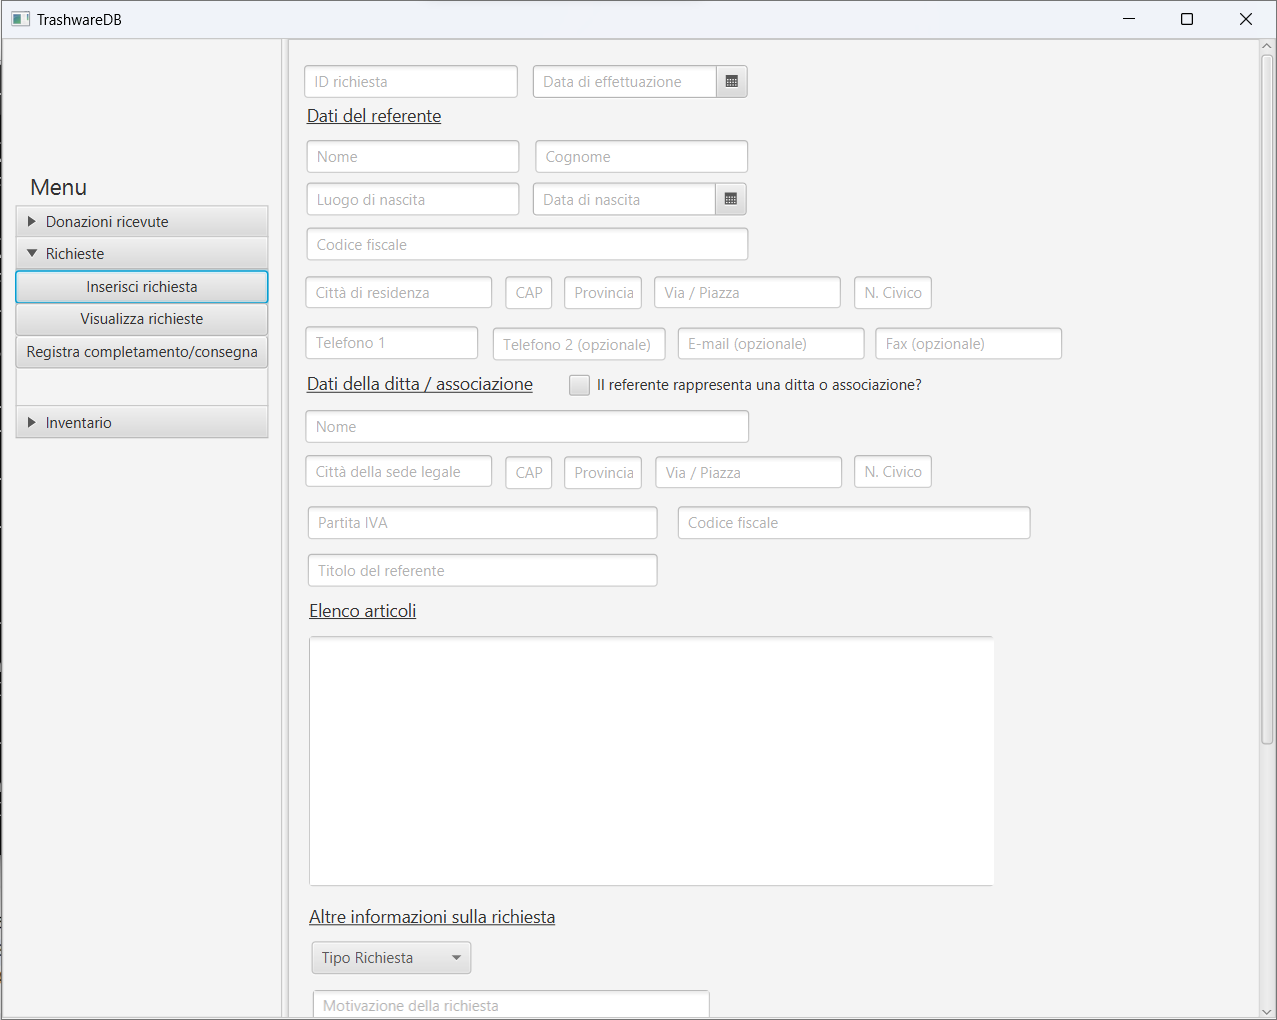
\includegraphics[width=\textwidth]{images/form-screen.png}
    \caption{Form di inserimento delle richieste.}
\end{figure}

\begin{figure}[H]
	\centering
	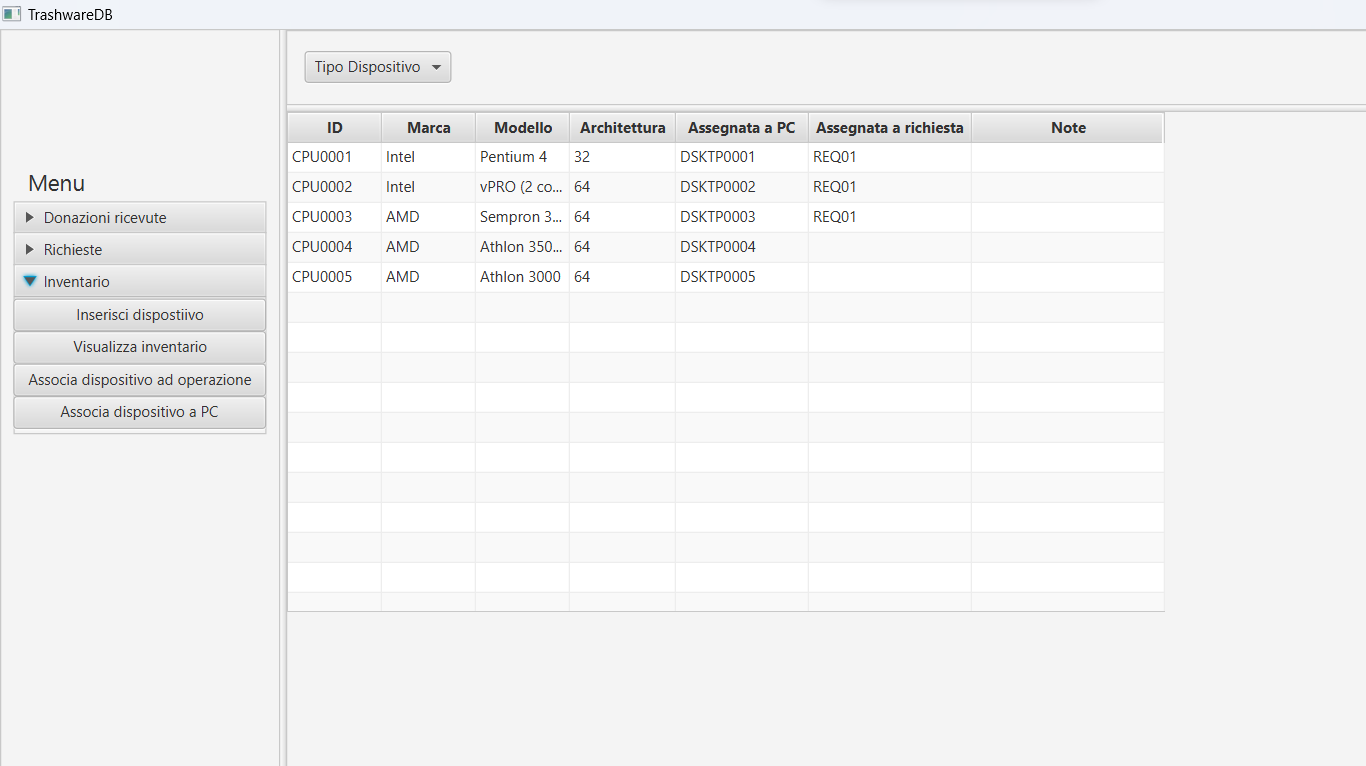
\includegraphics[width=\textwidth]{images/view-screen.png}
    \caption{Vista delle informazioni relative alle CPU.}
\end{figure}

\noindent L'aspetto grafico di ogni pagina è descritto dal corrispondente file FXML, mentre il suo comportamento è definito dal corrispondente GUI controller. \\
La parte di controller dell'applicazione è divisa in due parti: 
\\l'\texttt{OperationsController} espone i servizi legati alla gestione delle operazioni, mentre l'\texttt{InventoryController} espone i servizi legati alla gestione dell'inventario. \\
Ogni GUI controller utilizza i servizi forniti dall'opportuno controller per l'invio o la richiesta di dati. L'interazione con il database è poi effettuata mediante i servizi di Hibernate.

\section{Guida utente}

Coerentemente con le operazioni indicate nei requisiti, sono presenti form per la registrazione delle informazioni relative a donazioni, richieste, dispositivi e per l'associazione dei dispositivi alle operazioni, per l'associazione dei componenti/periferiche ai PC e per l'aggiornamento dello stato delle richieste. \\ 
Devono essere riempiti almeno i campi non opzionali, per poi procedere all'invio mediante il bottone "Inserisci" in basso a destra. A seguito dell'invio, viene mostrato un pop-up che riporta l'esito dell'inserimento, segnalando eventuali problemi. \\ 
Sono poi presenti le viste per la visualizzazione delle donazioni, delle richieste e dei dispositivi registrati. \\

\noindent L'applicazione prevede il seguente flusso di lavoro.
\begin{itemize}
    \item Quando viene ricevuta una donazione da parte del progetto, viene registrata mediante la pagina "Inserisci donazione".
    \item Quando i dispositivi ricevuti vengono analizzati, li si registra uno ad uno mediante gli opportuni form accessibili dalla pagina "Inserisci dispositivo".
    \begin{itemize}
        \item Per quanto riguarda i PC, si registrano prima le informazioni dei suoi componenti e delle eventuali periferiche associate, per poi registrare le informazioni del PC.
    \end{itemize}
    \item I dispositivi vengono associati alla donazione con cui sono stati ricevuti mediante la pagina "Associa dispositivo ad operazione".
    \item La pagina "Associa dispositivo a PC" permette di modificare i componenti associati ad un PC o di specificare/modificare le periferiche associate ad un PC desktop.
    \item Quando viene ricevuta una richiesta, la richiesta viene registrata mediante la pagina "Inserisci richiesta". I dispositivi legati alla richiesta vengono poi associati ad essa mediante la pagina "Associa dispositivo ad operazione", sia esso un dispositivo scelto dall'inventario per essere donato o un dispositivo restituito per la manutenzione.
    \item Quando i dispositivi legati ad una richiesta sono pronti o consegnati, si registra il completamento o la consegna mediante la pagina "Registra completamento/consegna".
    \item In qualsiasi momento, si possono visualizzare donazioni, richieste e dispositivi in inventario mediante le pagine "Visualizza donazioni", Visualizza richieste" e "Visualizza inventario".
\end{itemize}

\noindent Si segnala che nella vista delle richieste è necessario selezionare quali richieste si vogliono visualizzare in base allo stato corrente, mentre per ottenere il form o la vista della categoria di dispositivi desiderata è necessario specificarla. In tutti questi casi, tali parametri vengono specificati selezionando l'opportuna voce del menù posto nella parte alta della pagina. \\

%------------------------------------------------------

\end{document}
